% \documentclass{article}
\documentclass[../../outputs/main.tex]{subfiles}

% Any packages or configurations specific to this section
\usepackage{lipsum}
\usepackage{graphicx}

\begin{document}

In the following subsections, the proposed algorithm is compared against the centralized (MPCOPF) algorithm in terms of resultant optimal control variables, optimality gap in objective function and computational performance. Secondly, the resultant control variables are tested for ACOPF feasiblity against OpenDSS. \Cref{subsec:simulationResults} describes the comparison over a $5$ time-period horizon with an additional focus on describing the workflow of the MPDOPF algorithm. \Cref{subsec:scalabilityAnalysis} describes the comparsion over a $10$ time-period horizon to test for the scalability of the MPDOPF algorithm.

\subsection{Simulation Results} \label{subsec:simulationResults}
% Case 1: centralized OPF with battery
% Case 2: ENApp based distributed OPF with battery

\Cref{table:opt-5-20-30} represents a comparison between MPCOPF and MPDOPF in their problem scope, results and computational performance.

\subsubsection{Biggest Subproblem vs Computational Performance}
This first section of the table, 'Biggest subproblem' provides specifics of the `computational bottleneck' encountered by either algorithm during its course. As described in \Cref{subsec:ENApp}, the bottleneck represents the OPF subproblem which is computationally the most intensive, and thus is a key indicator of the expected time the algorithm will take to complete. As can be seen in the third section 'Computation', there is more than a $10$x speedup in computation time with MPDOPF, despite the fact that $5$ such iterations were performed, totalling to $20$ OPF calls over the $4$ areas of the Test System.      

\subsubsection{Optimality of Objective Function and Control Values}
The second section of the table 'Simulation results' showcases that MPDOPF provides virtually zero optimality gap (same values for Substation Power Cost, the objective function). Interestingly, the values of the control variable themselves, prominently, there is a significant difference in the suggested optimal reactive power control values for inverters associated with DERs and Batteries (results aggregated over all components over the horizon for conciseness). This highlights the fact that for a nonconvex nonlinear optimization problem may not necessarily have a unique global optimal point. 

\begin{table}[h!] % MPCOPF vs MPDOPF for T = 5
    \centering
    \caption{Comparative analyses between MPCOPF and MPDOPF - $5$ time-period horizon}
    \begin{tabular}{|l|c|c|}
    \hline
    \textbf{Metric} & \textbf{MPCOPF} & \textbf{MPDOPF} \\ \hline
    Biggest subproblem & \multicolumn{2}{c|}{} \\ \hline
    \quad Decision variables & {3150} & {1320} \\ \hline
    \quad Linear constraints & {5831} & {2451} \\ \hline
    \quad Nonlinear constraints & {635} & {265} \\ \hline
    Simulation results  & \multicolumn{2}{c|}{} \\ \hline
    \quad Substation power cost (\$) & 576.31 & 576.30 \\ \hline
    \quad Substation real power (kW) & 4308.28 & 4308.14 \\ \hline
    \quad Line loss (kW) & 75.99 & 76.12 \\ \hline
    \quad Substation reactive power (kVAR) & 574.18 & 656.24 \\ \hline
    \quad PV reactive power (kVAR) & 116.92 & 160.64 \\ \hline
    \quad Battery reactive power (kVAR) & 202.73 & 76.01 \\ \hline
    Computation  & \multicolumn{2}{c|}{} \\ \hline
    \quad Number of Iterations & - & 5 \\ \hline
    \quad Total Simulation Time (s) & 521.25 & 49.87 \\ \hline
    \end{tabular}
    \label{table:opt-5-20-30}
\end{table}

\Cref{table:feas-5-20-30} showcases the feasiblity of the control values suggested by the MPDOPF algorithm. First section 'Full horizon' describes the respective output variables for the entire horizon from MPDOPF and OpenDSS. Second section 'Max. all-time discrepancy' stores the highest discrepancy between key state/output variables for all components across at any time-period between MPDOPF and OpenDSS. In both sections, the discrepancies are small enough to warrant feasiblity of the obtained solution. 

\begin{table}[h!]
    \centering
    \caption{ACOPF feasibility analyses - $5$ time-period horizon}
    \begin{tabular}{|l|c|c|}
    \hline
    \textbf{Metric} & \textbf{MPDOPF} & \textbf{OpenDSS} \\ \hline
    Full horizon  & \multicolumn{2}{c|}{} \\ \hline
    \quad Substation real power (kW) & 4308.14 & 4308.35 \\ \hline
    \quad Line loss (kW) & 76.12 & 76.09 \\ \hline
    \quad Substation reactive power (kVAR) & 656.24 & 652.49 \\ \hline
    Max. all-time discrepancy & \multicolumn{2}{c|}{} \\ \hline
    \quad Voltage (pu) & \multicolumn{2}{c|}{0.0002} \\ \hline
    \quad Line loss (kW) & \multicolumn{2}{c|}{0.0139} \\ \hline
    \quad Substation power (kW) & \multicolumn{2}{c|}{0.3431} \\ \hline
    \end{tabular}
    \label{table:feas-5-20-30}
\end{table}

To ensure that the complementarity of charging and discharging of batteries are being respected despite not using integer constraints, the charging/discharging profiles for batteries were checked, and indeed that is the case. \Cref{fig:batt-plot-dopf-5-20-30-genCost} is shown as one example.

\begin{figure}[h!]
    \centering
    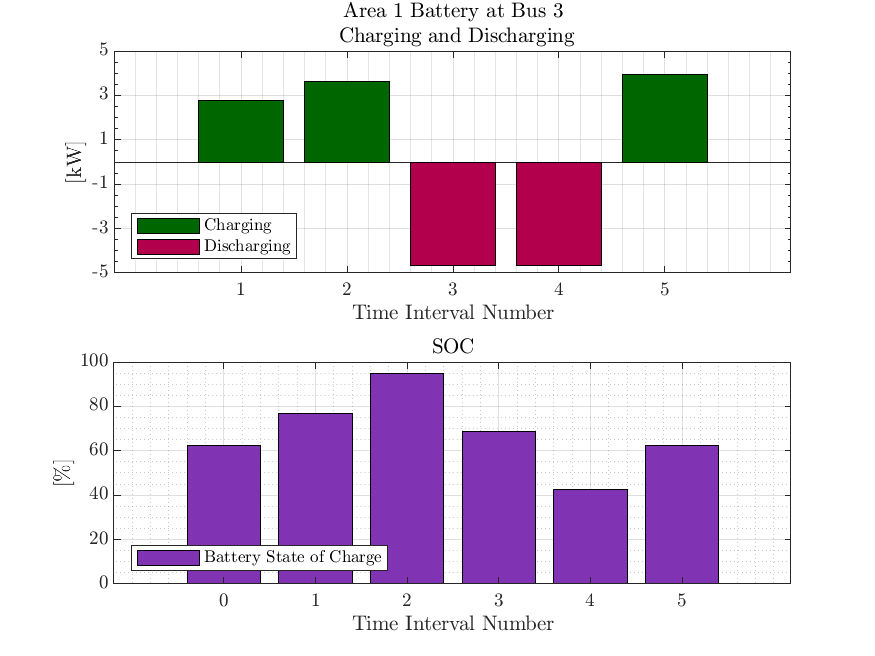
\includegraphics[width=\linewidth]{../figures/T5-pv20-batt30-genCost/dopf/BatteryPlots/macroItr_5_genCost_Battery_1_alpha_0.001.png}
    \caption{Charging-Discharging and SOC graphs for Battery at Bus 3 located in Area 1 obtained by MPDOPF}
    \label{fig:batt-plot-dopf-5-20-30-genCost}
\end{figure}

The workflow of the MPDOPF algorithm, which involves exchange of boundary variables between parent-child area pairs, can be seen in the convergence plots in \Cref{fig:convergenceCurves-5-20-30}.

% \begin{figure*}[h!] % convergence curves
%     \centering
%     % Row 1
%     \begin{subfigure}[b]{0.3\textwidth}
%         \centering
%         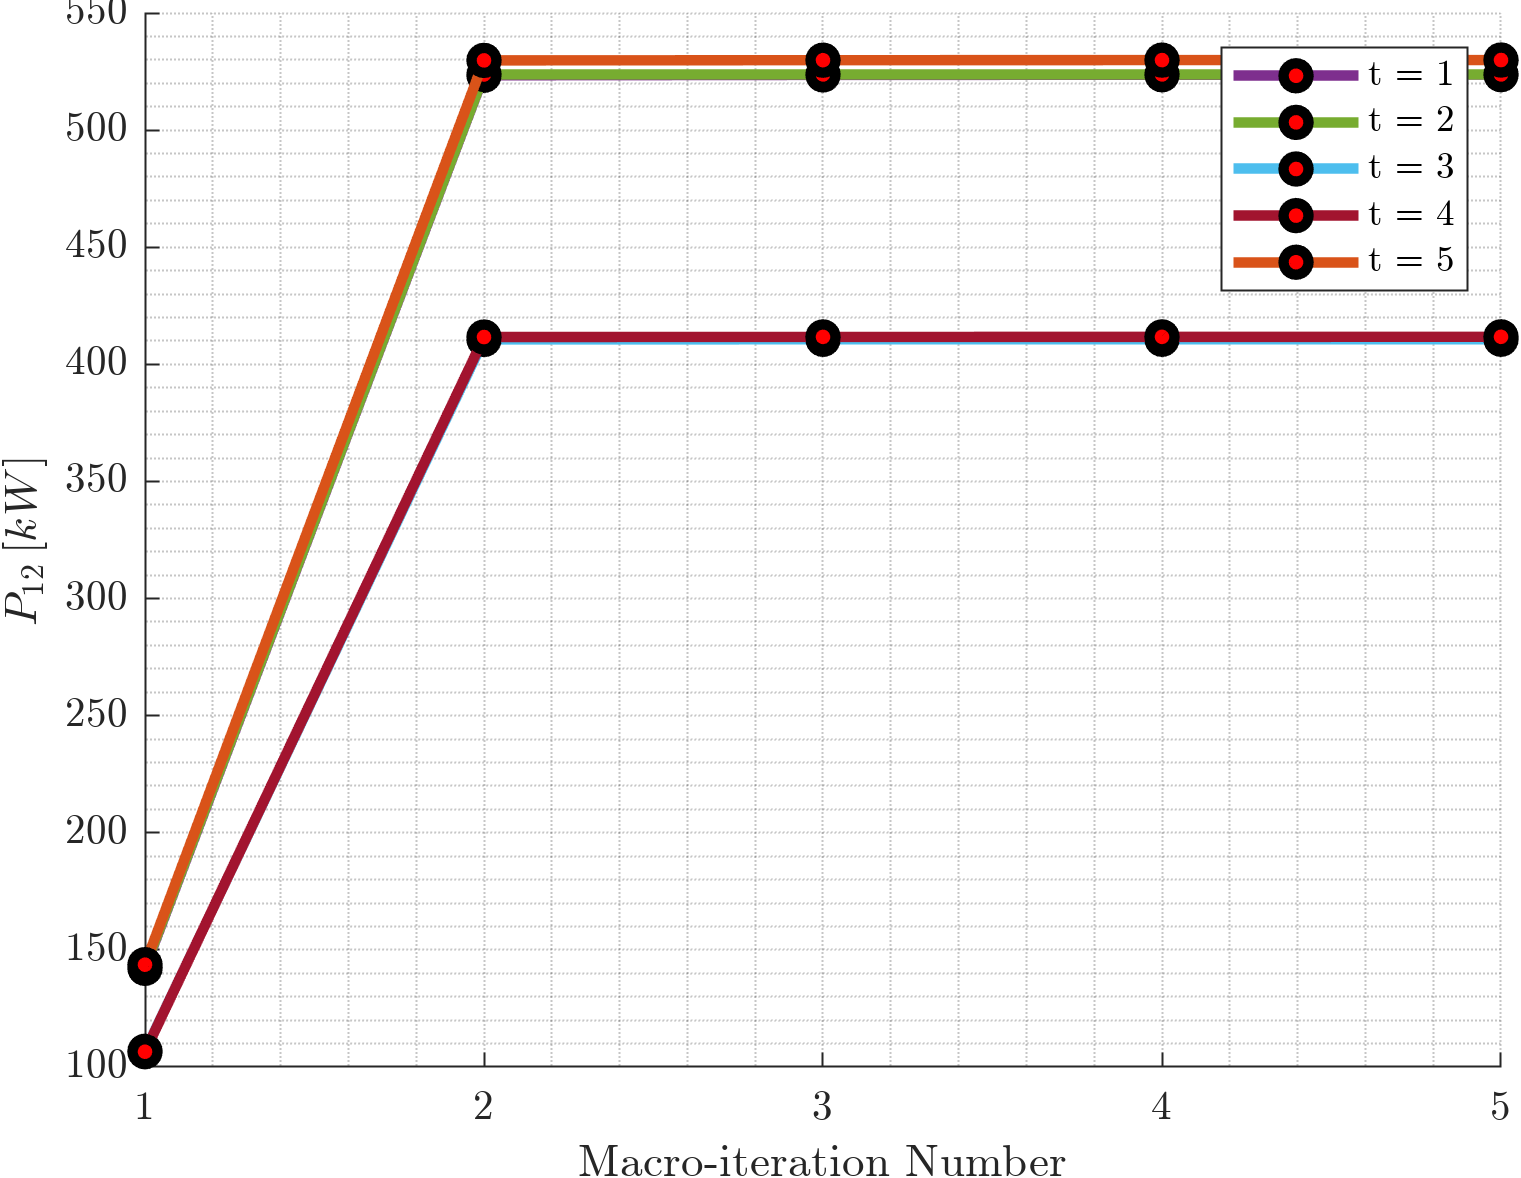
\includegraphics[width=\textwidth]{../figures/T5-pv20-batt30-genCost/dopf/convergenceCurves/BoundaryRealPower_vs_t_vs_macroItr_T_5_Areas_1_2_genCost_pv_20_batt_30_crop.png}
%         \caption{\scriptsize Real Power flowing from Area $1$ into Area $2$}
%         \label{fig:real_power_1_2}
%     \end{subfigure}
%     \hfill
%     \begin{subfigure}[b]{0.3\textwidth}
%         \centering
%         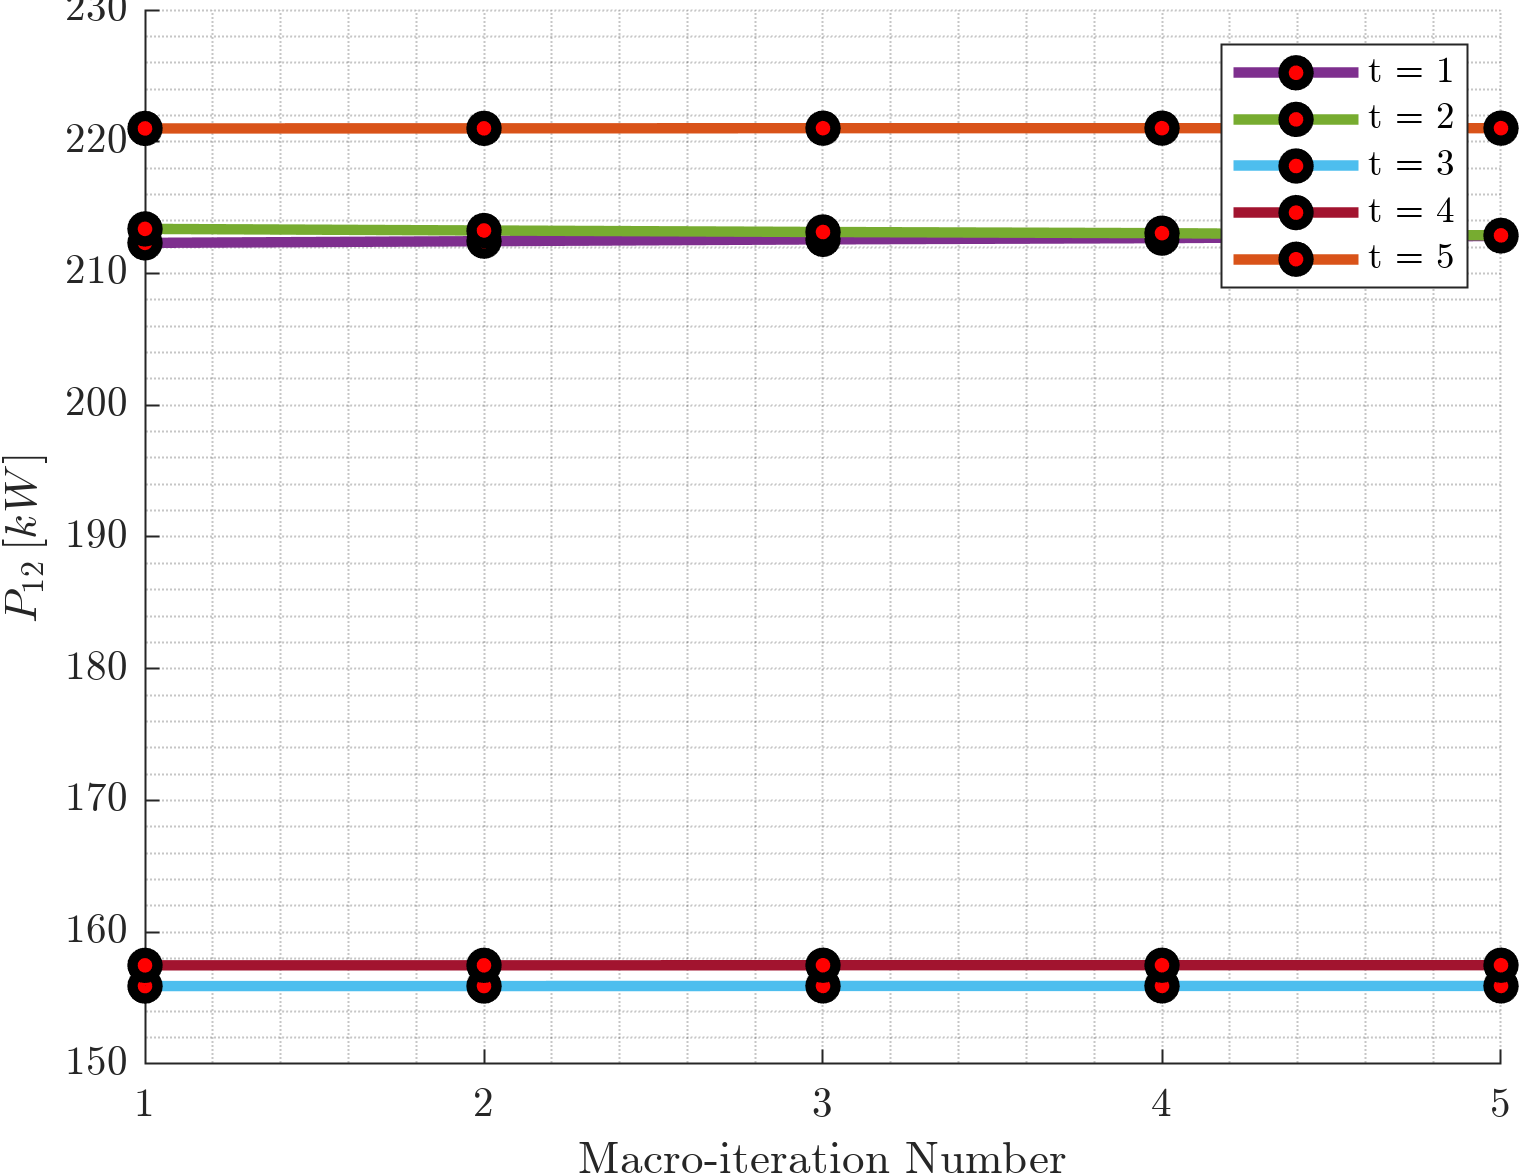
\includegraphics[width=\textwidth]{../figures/T5-pv20-batt30-genCost/dopf/convergenceCurves/BoundaryRealPower_vs_t_vs_macroItr_T_5_Areas_1_3_genCost_pv_20_batt_30_crop.png}
%         \caption{\scriptsize Real Power flowing from Area $1$ into Area $3$}
%         \label{fig:real_power_1_3}
%     \end{subfigure}
%     \hfill
%     \begin{subfigure}[b]{0.3\textwidth}
%         \centering
%         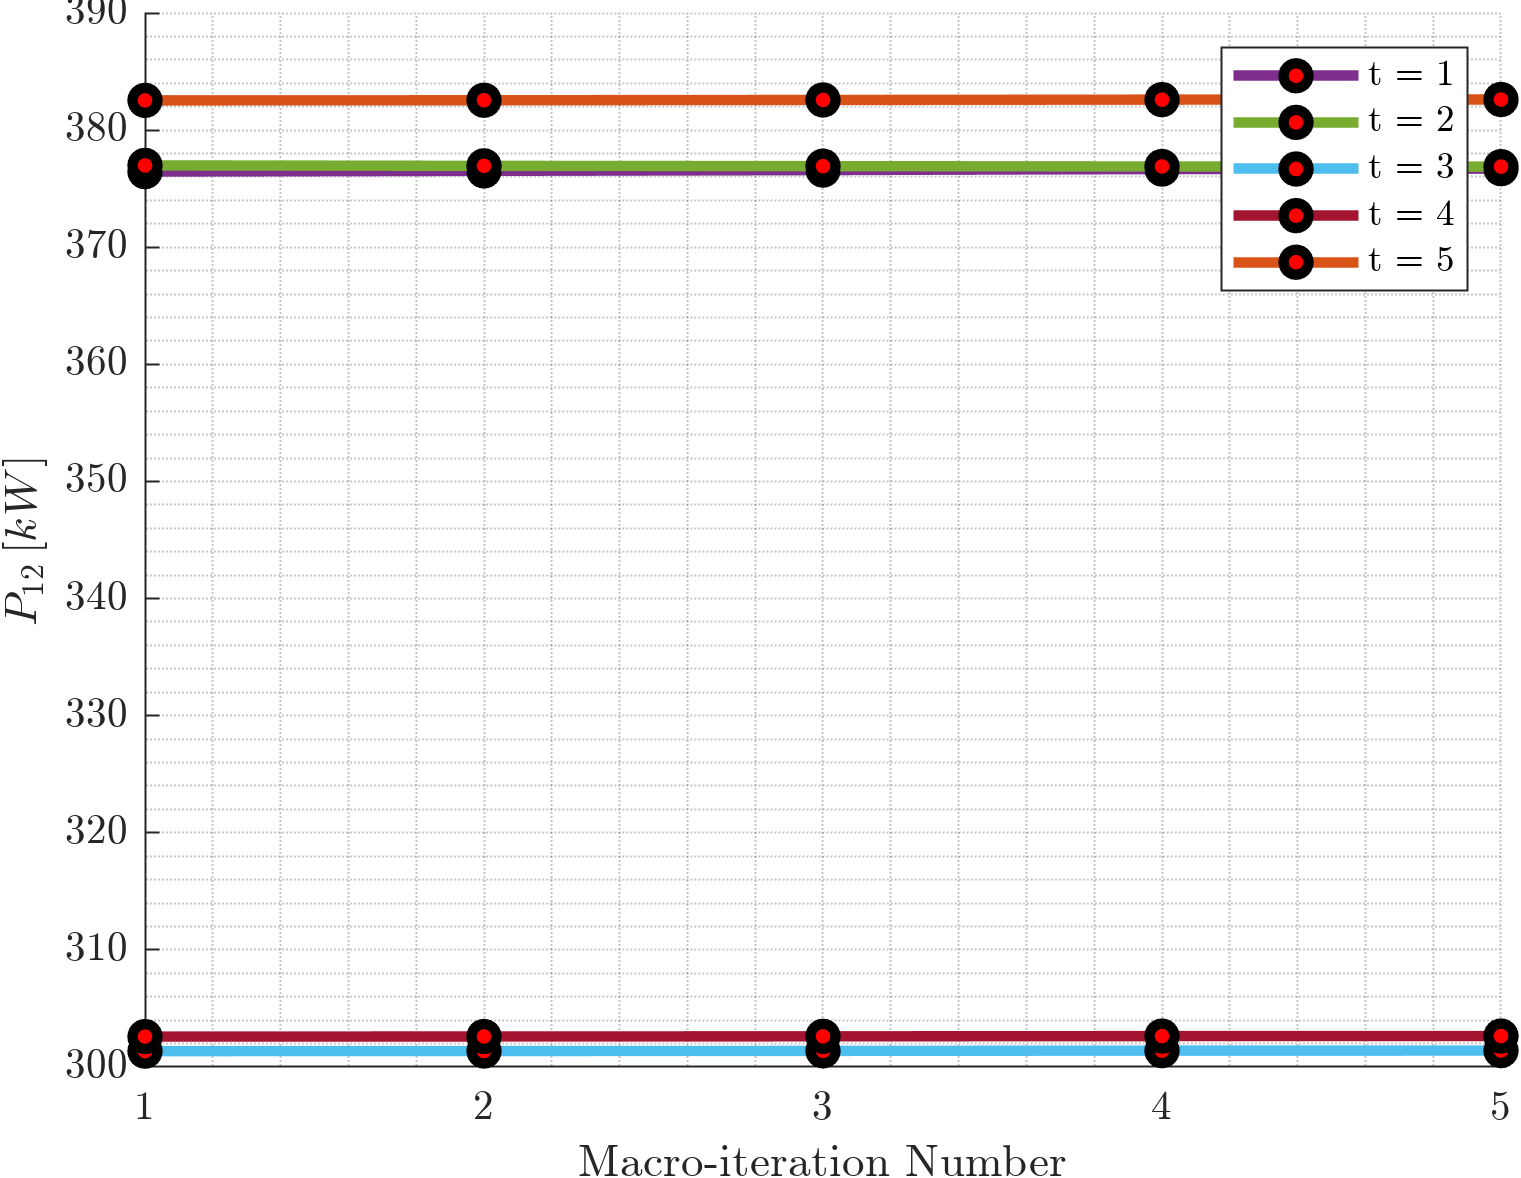
\includegraphics[width=\textwidth]{../figures/T5-pv20-batt30-genCost/dopf/convergenceCurves/BoundaryRealPower_vs_t_vs_macroItr_T_5_Areas_2_4_genCost_pv_20_batt_30_crop.png}
%         \caption{\scriptsize Real Power flowing from Area $2$ into Area $4$}
%         \label{fig:real_power_2_4}
%     \end{subfigure}
    
%     % Row 2
%     \begin{subfigure}[b]{0.3\textwidth}
%         \centering
%         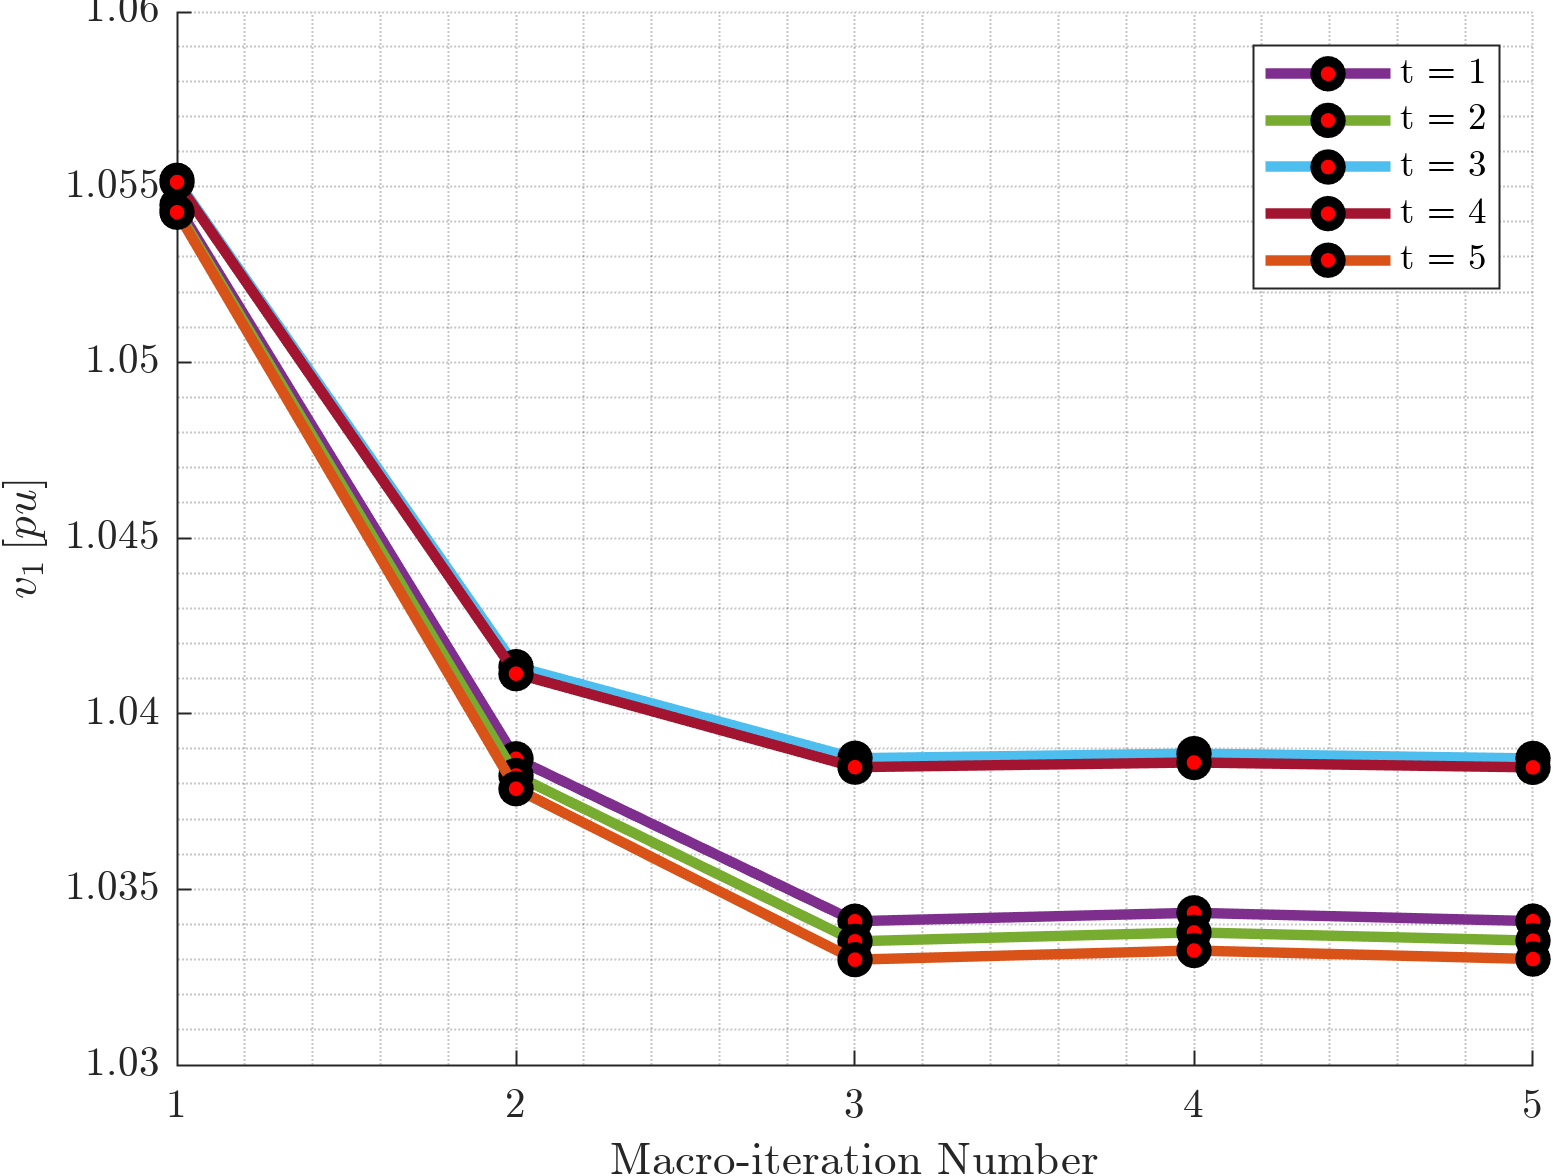
\includegraphics[width=\textwidth]{../figures/T5-pv20-batt30-genCost/dopf/convergenceCurves/BoundaryVoltage_vs_t_vs_macroItr_T_5_Areas_1_2_genCost_pv_20_batt_30_crop.png}
%         \caption{\scriptsize Voltage at the PoI of Area $1$ and Area $2$}
%         \label{fig:voltage_1_2}
%     \end{subfigure}
%     \hfill
%     \begin{subfigure}[b]{0.3\textwidth}
%         \centering
%         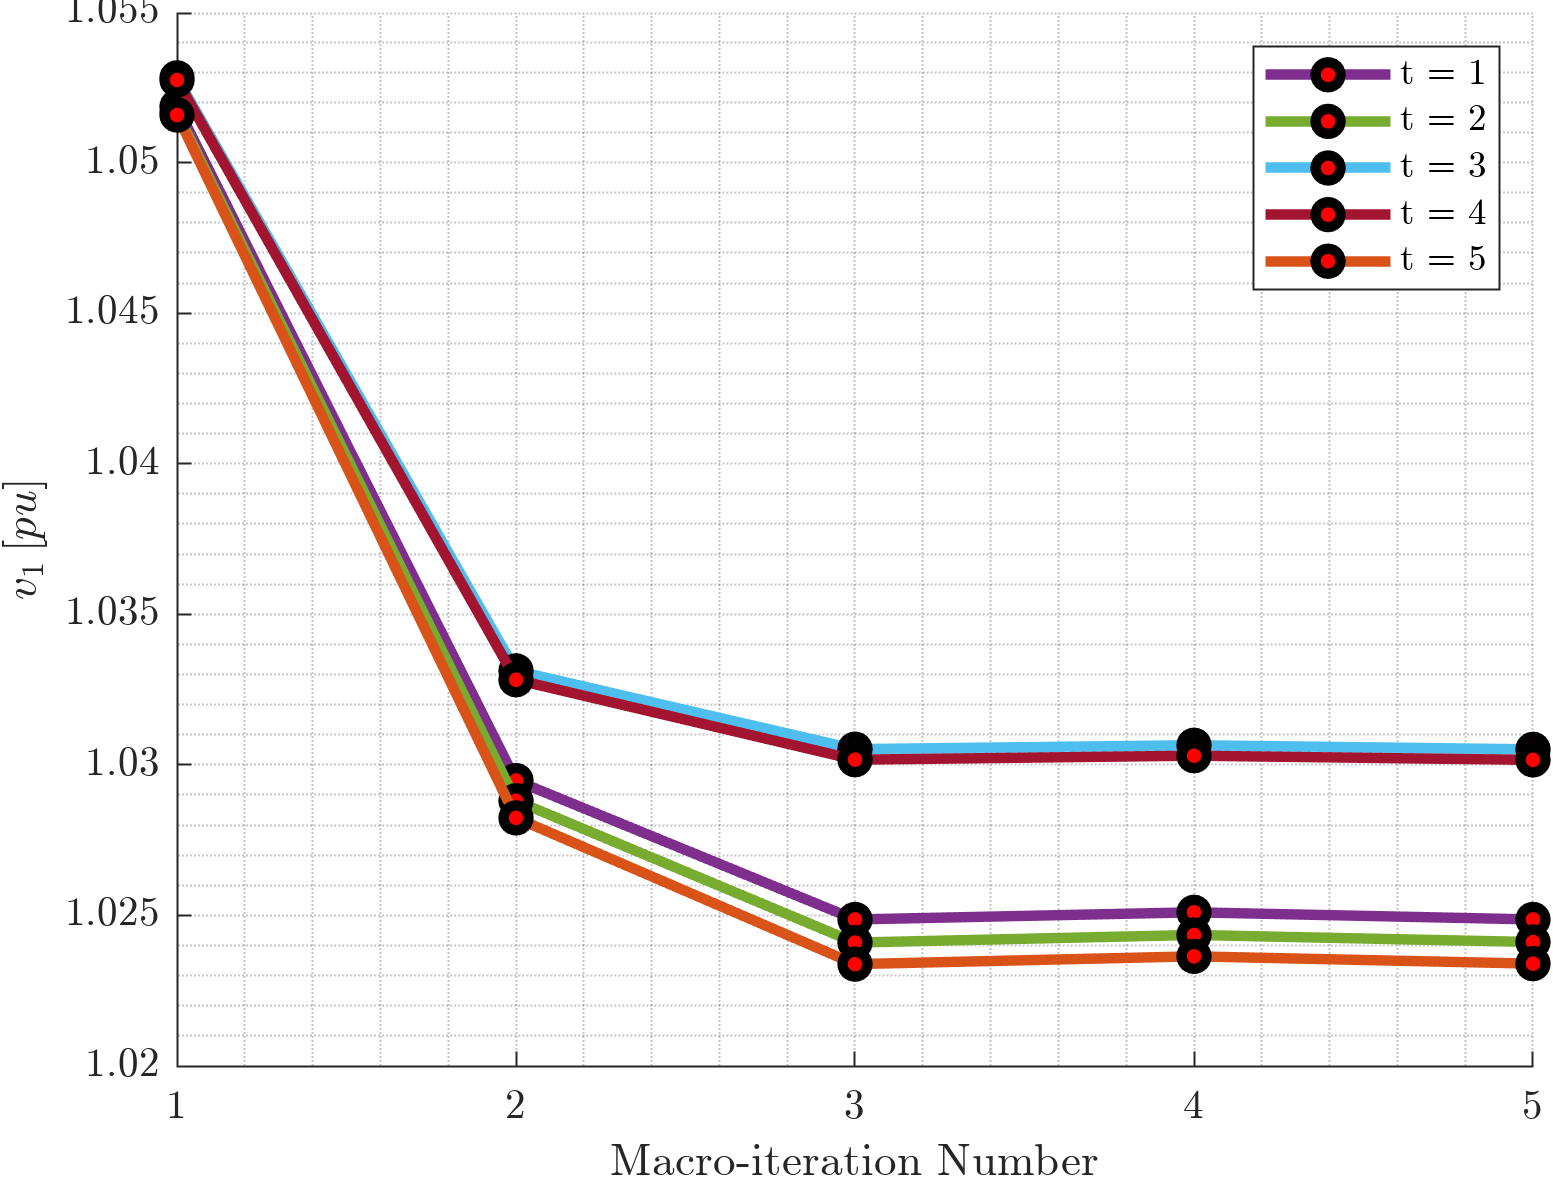
\includegraphics[width=\textwidth]{../figures/T5-pv20-batt30-genCost/dopf/convergenceCurves/BoundaryVoltage_vs_t_vs_macroItr_T_5_Areas_1_3_genCost_pv_20_batt_30_crop.png}
%         \caption{\scriptsize Voltage at the PoI of Area $1$ and Area $3$}
%         \label{fig:voltage_1_3}
%     \end{subfigure}
%     \hfill
%     \begin{subfigure}[b]{0.3\textwidth}
%         \centering
%         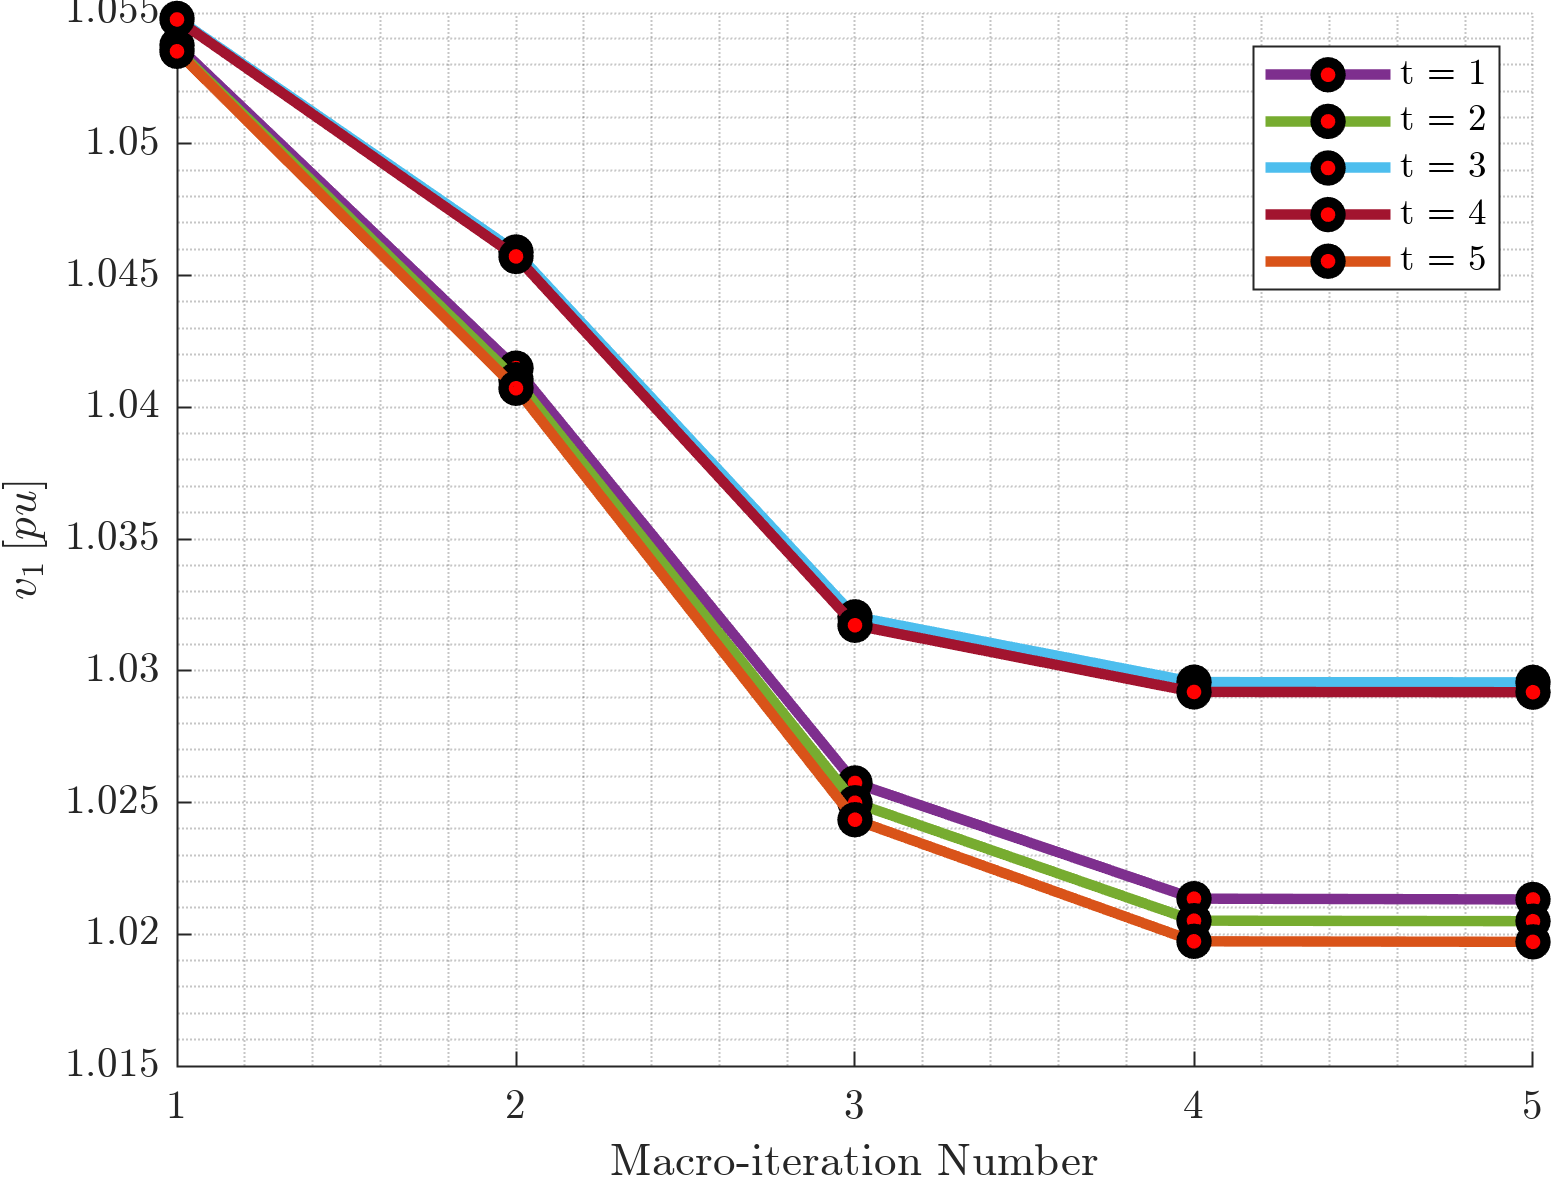
\includegraphics[width=\textwidth]{../figures/T5-pv20-batt30-genCost/dopf/convergenceCurves/BoundaryVoltage_vs_t_vs_macroItr_T_5_Areas_2_4_genCost_pv_20_batt_30_crop.png}
%         \caption{\scriptsize Voltage at the PoI of Area $2$ and Area $4$}
%         \label{fig:voltage_2_4}
%     \end{subfigure}

%     \caption{Convergence of Boundary variables with every iteration. Each plot represents a particular variable exchanged between a pair of connected areas. Each line graph within a plot represents a particular time period.}
%     \label{fig:convergenceCurves-5-20-30}
% \end{figure*}

% \begin{figure*}[h] % convergence curves
%     \centering
%     % Row 1
%     \begin{subfigure}[b]{0.3\textwidth}
%         \centering
%         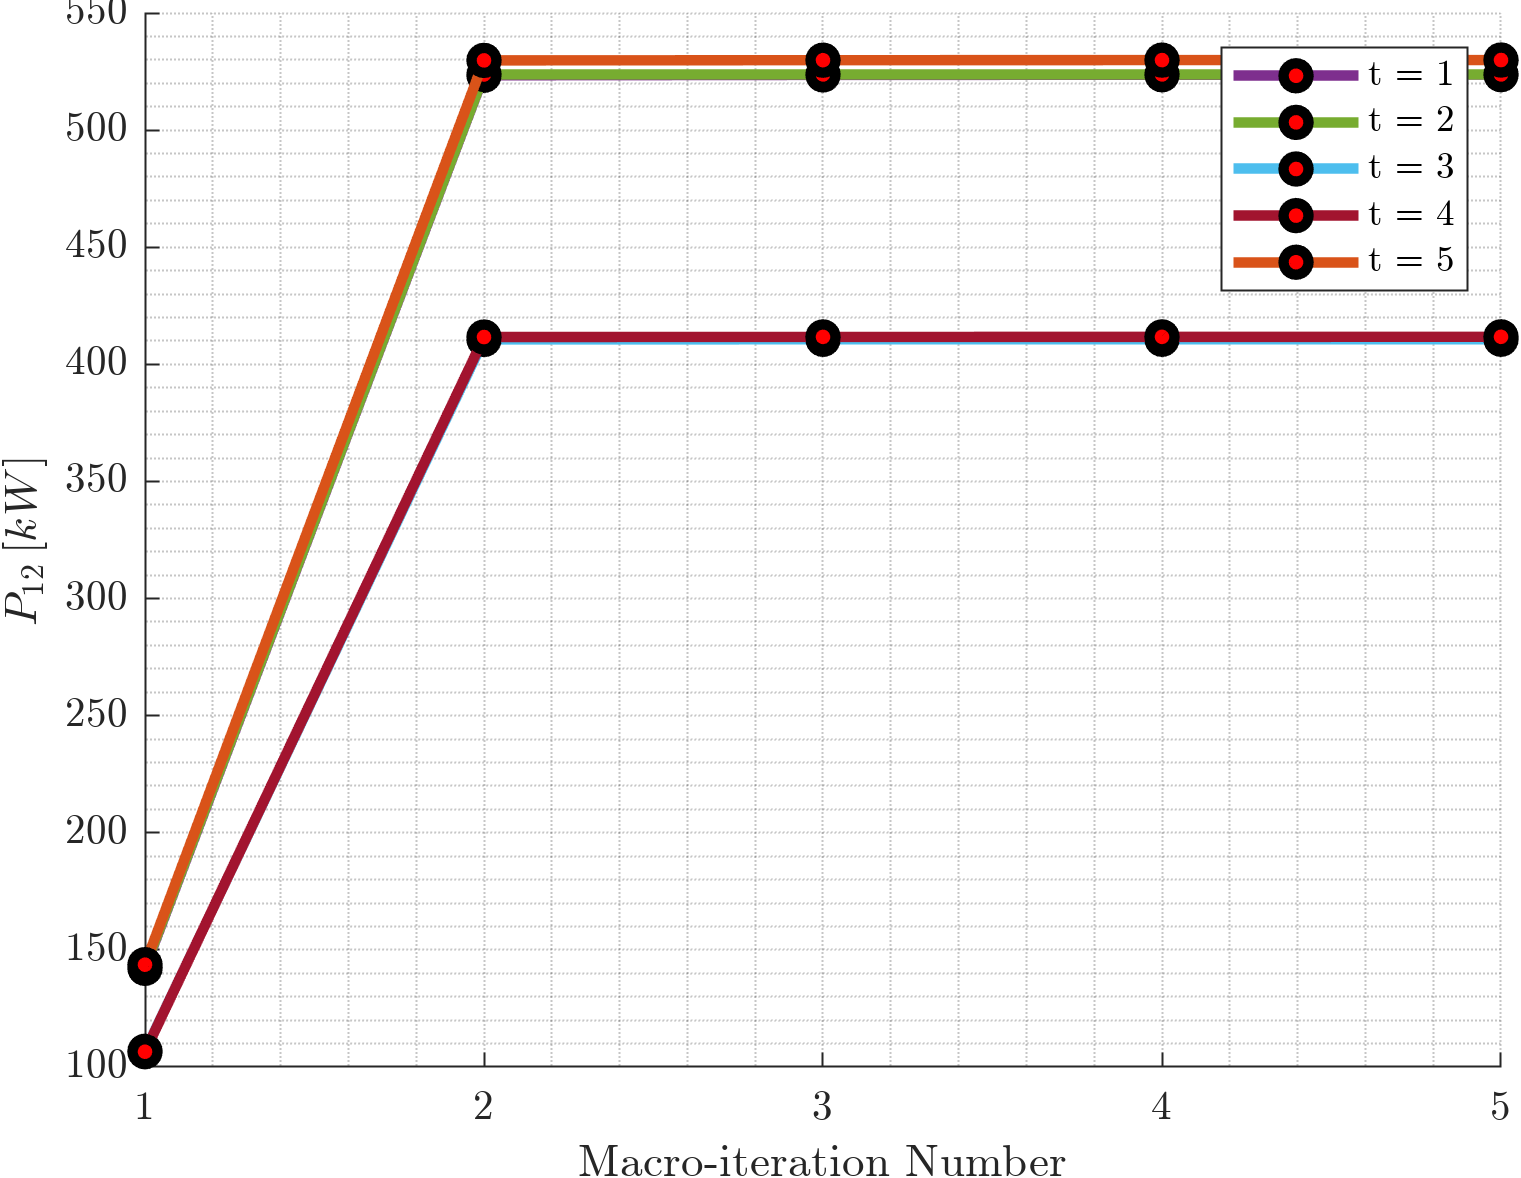
\includegraphics[scale=0.3]{../figures/T5-pv20-batt30-genCost/dopf/convergenceCurves/BoundaryRealPower_vs_t_vs_macroItr_T_5_Areas_1_2_genCost_pv_20_batt_30_crop.png}
%         \caption{\scriptsize Real Power flowing from Area $1$ into Area $2$}
%         \label{fig:real_power_1_2}
%     \end{subfigure}
%     \hfill
%     \begin{subfigure}[b]{0.3\textwidth}
%         \centering
%         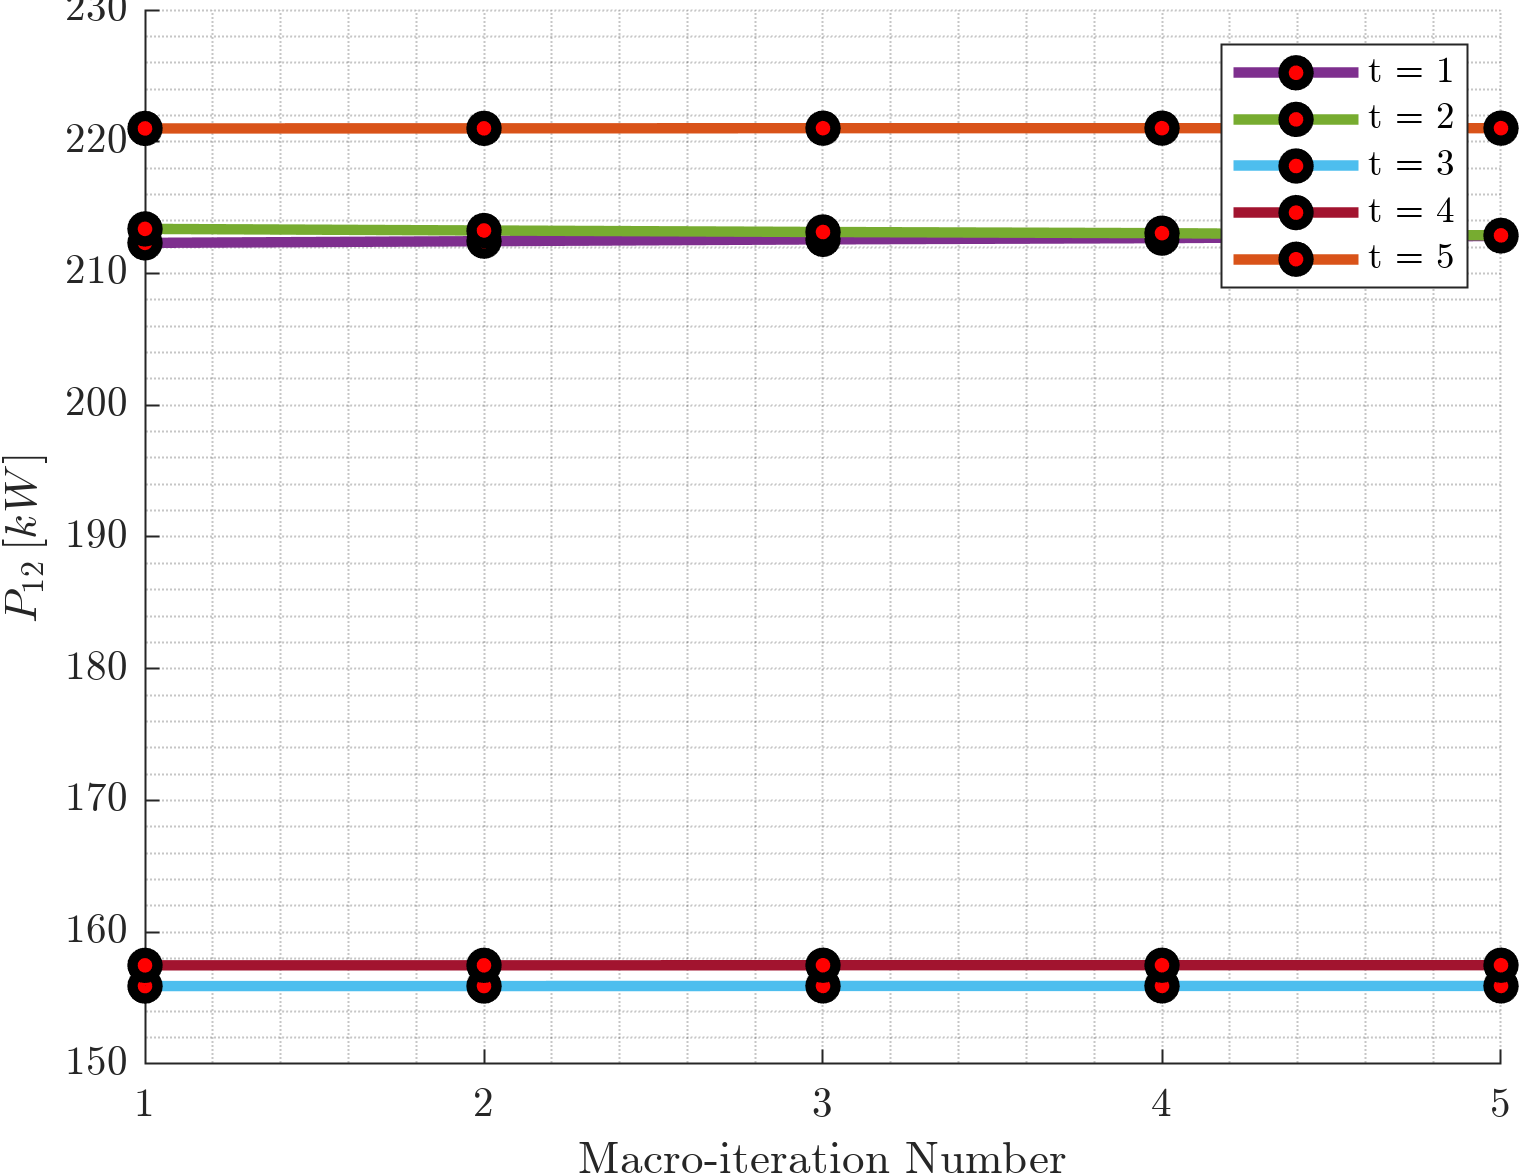
\includegraphics[scale=0.3]{../figures/T5-pv20-batt30-genCost/dopf/convergenceCurves/BoundaryRealPower_vs_t_vs_macroItr_T_5_Areas_1_3_genCost_pv_20_batt_30_crop.png}
%         \caption{\scriptsize Real Power flowing from Area $1$ into Area $3$}
%         \label{fig:real_power_1_3}
%     \end{subfigure}
%     \hfill
%     \begin{subfigure}[b]{0.3\textwidth}
%         \centering
%         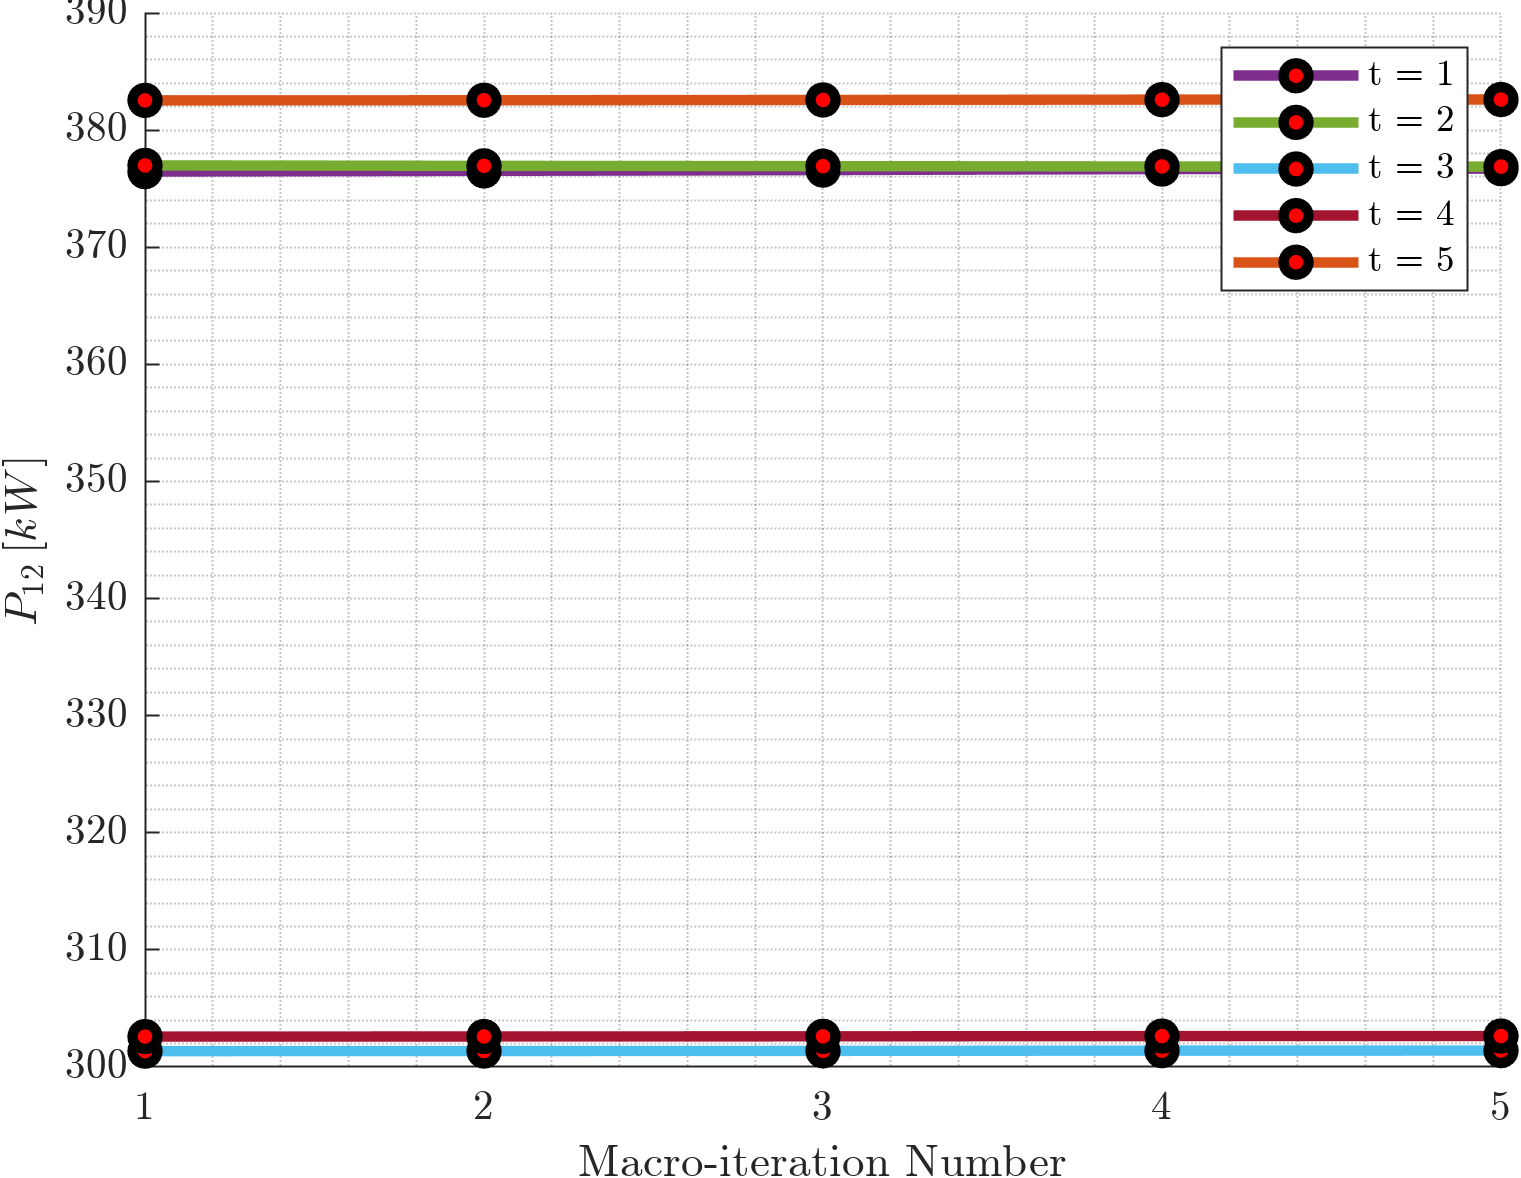
\includegraphics[scale=0.3]{../figures/T5-pv20-batt30-genCost/dopf/convergenceCurves/BoundaryRealPower_vs_t_vs_macroItr_T_5_Areas_2_4_genCost_pv_20_batt_30_crop.png}
%         \caption{\scriptsize Real Power flowing from Area $2$ into Area $4$}
%         \label{fig:real_power_2_4}
%     \end{subfigure}
    
%     % Row 2
%     \begin{subfigure}[b]{0.3\textwidth}
%         \centering
%         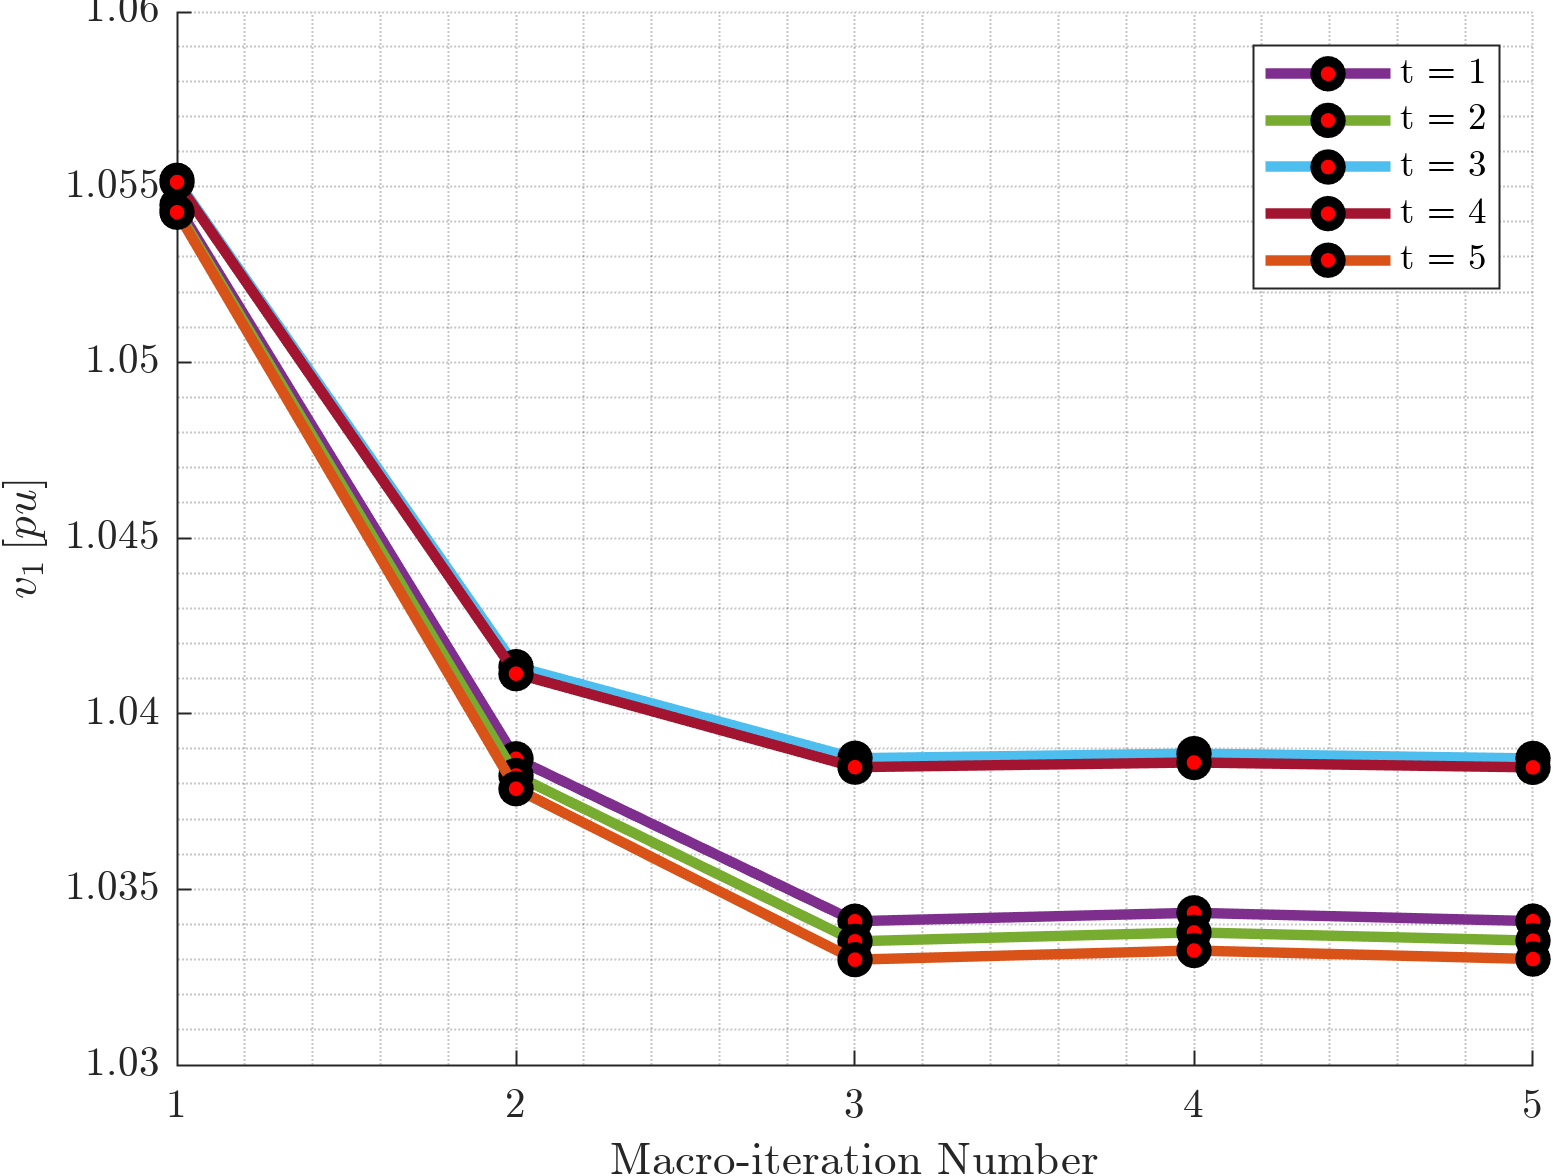
\includegraphics[scale=0.3]{../figures/T5-pv20-batt30-genCost/dopf/convergenceCurves/BoundaryVoltage_vs_t_vs_macroItr_T_5_Areas_1_2_genCost_pv_20_batt_30_crop.png}
%         \caption{\scriptsize Voltage at the PoI of Area $1$ and Area $2$}
%         \label{fig:voltage_1_2}
%     \end{subfigure}
%     \hfill
%     \begin{subfigure}[b]{0.3\textwidth}
%         \centering
%         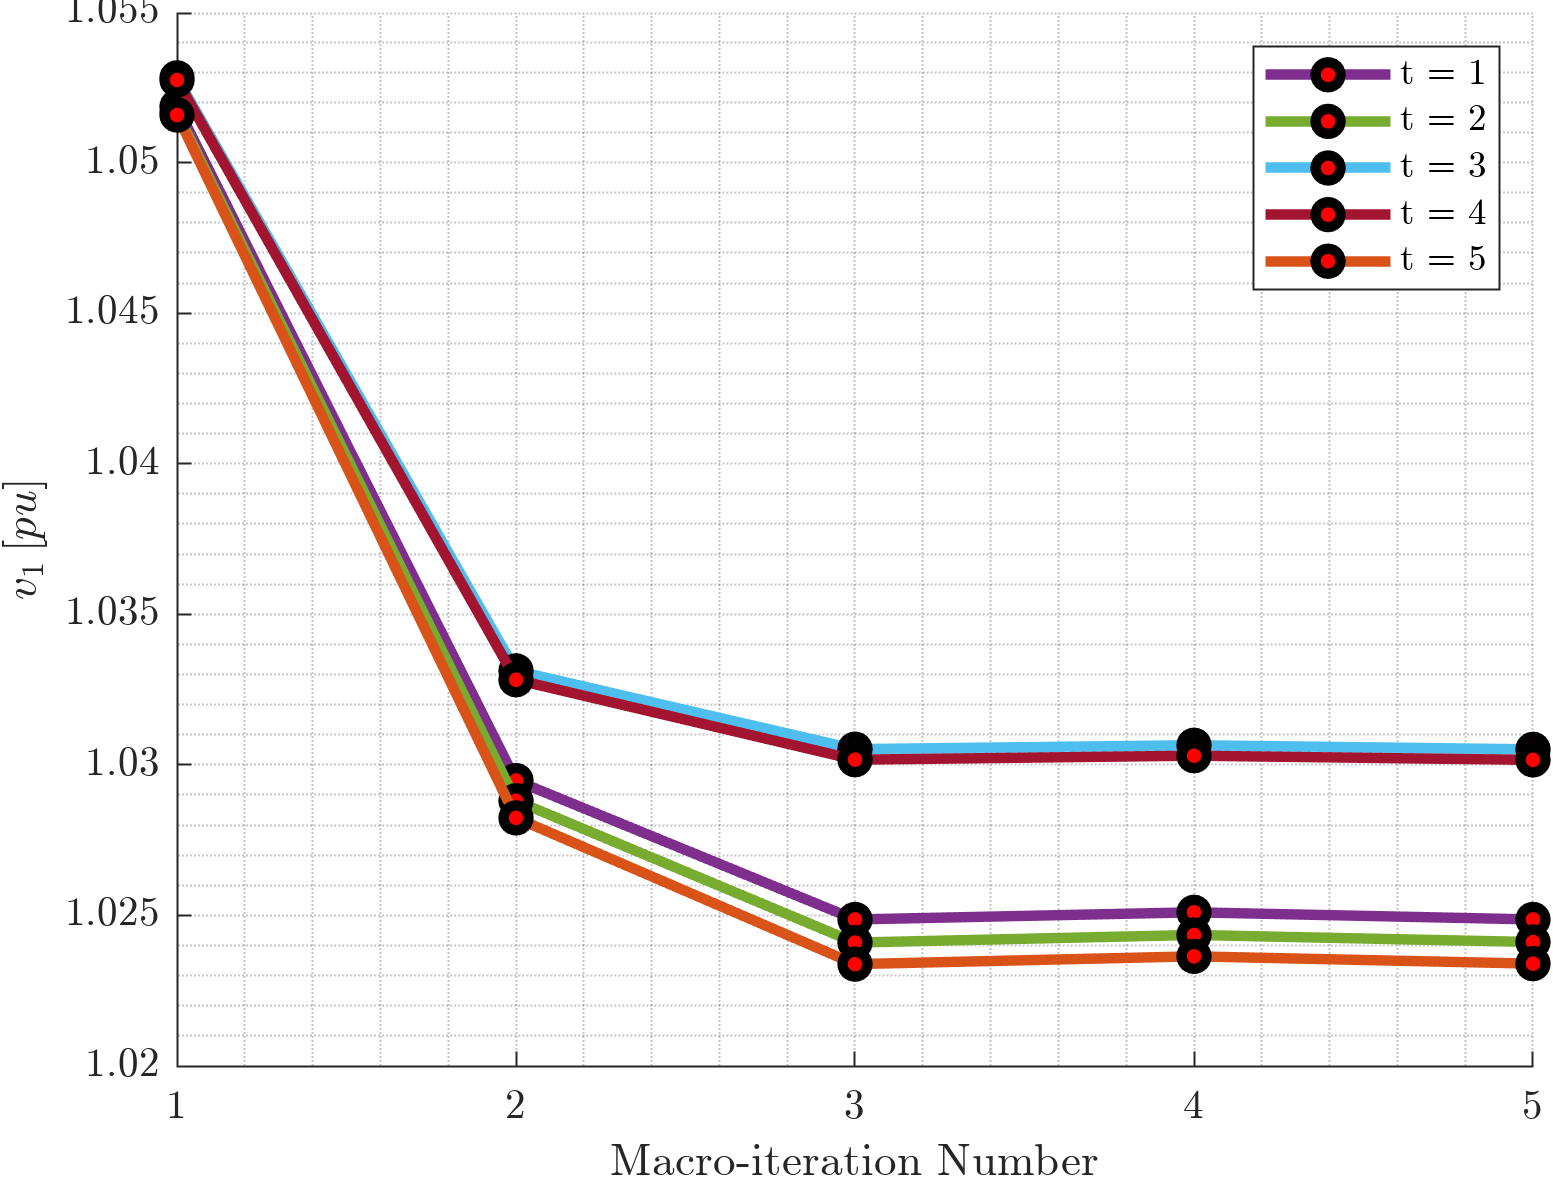
\includegraphics[scale=0.3]{../figures/T5-pv20-batt30-genCost/dopf/convergenceCurves/BoundaryVoltage_vs_t_vs_macroItr_T_5_Areas_1_3_genCost_pv_20_batt_30_crop.png}
%         \caption{\scriptsize Voltage at the PoI of Area $1$ and Area $3$}
%         \label{fig:voltage_1_3}
%     \end{subfigure}
%     \hfill
%     \begin{subfigure}[b]{0.3\textwidth}
%         \centering
%         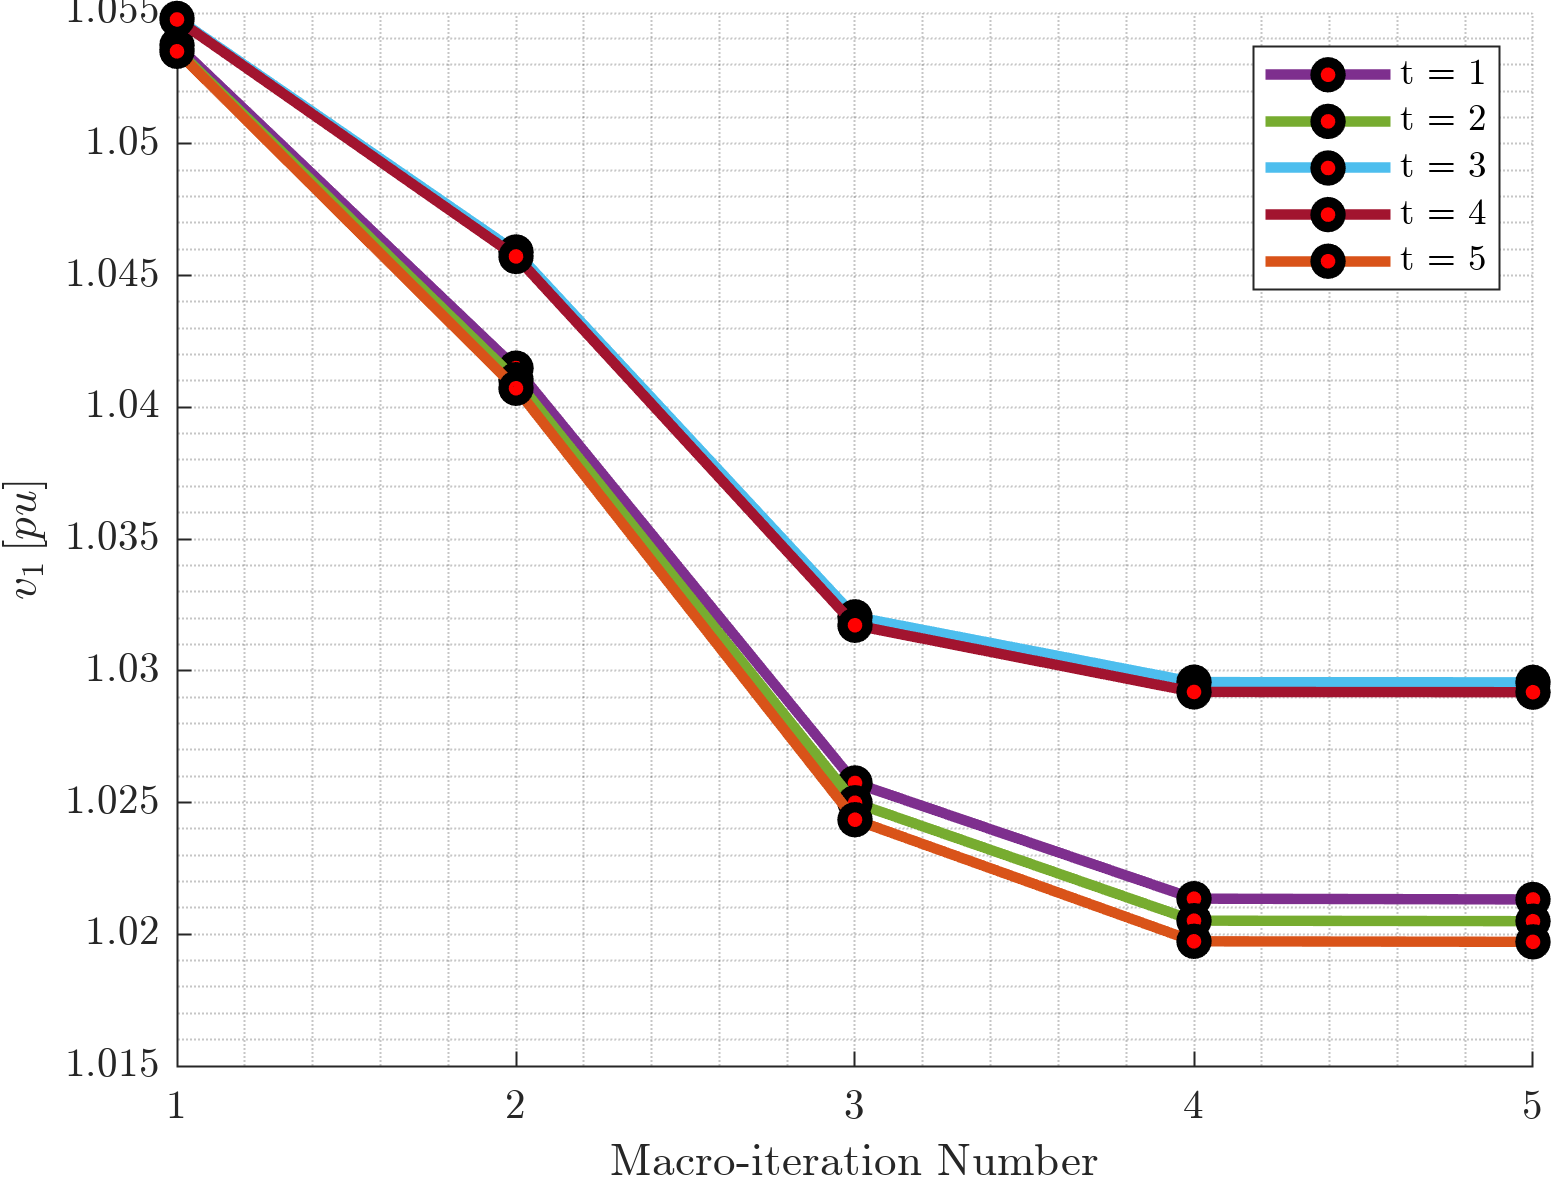
\includegraphics[scale=0.3]{../figures/T5-pv20-batt30-genCost/dopf/convergenceCurves/BoundaryVoltage_vs_t_vs_macroItr_T_5_Areas_2_4_genCost_pv_20_batt_30_crop.png}
%         \caption{\scriptsize Voltage at the PoI of Area $2$ and Area $4$}
%         \label{fig:voltage_2_4}
%     \end{subfigure}

%     \caption{Convergence of Boundary variables with every iteration. Each plot represents a particular variable exchanged between a pair of connected areas. Each line graph within a plot represents a particular time period.}
%     \label{fig:convergenceCurves-5-20-30}
% \end{figure*}

% \begin{figure}[H] % convergence curves
%     \centering
%     % Row 1
%     \begin{subfigure}[b]{0.3\textwidth}
%         \centering
%         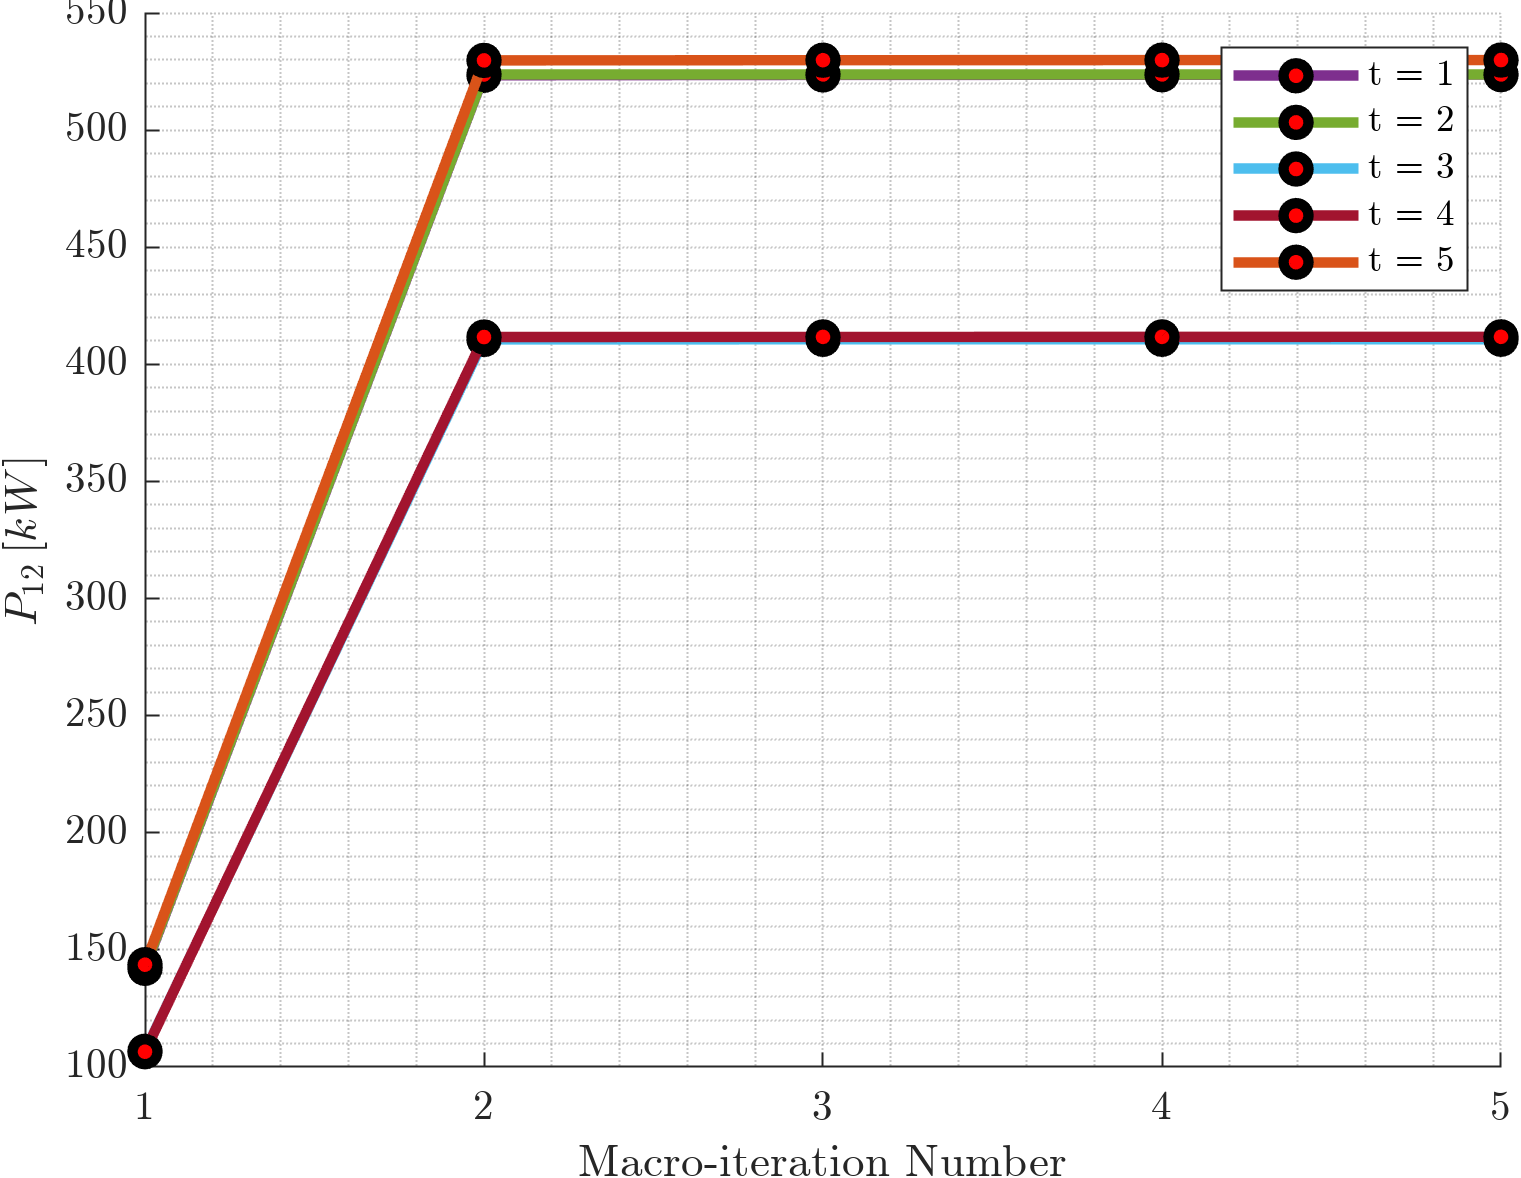
\includegraphics[width=\textwidth,height=0.6\textwidth]{../figures/T5-pv20-batt30-genCost/dopf/convergenceCurves/BoundaryRealPower_vs_t_vs_macroItr_T_5_Areas_1_2_genCost_pv_20_batt_30_crop.png}
%         \caption{\scriptsize Real Power flowing from Area $1$ into Area $2$}
%         \label{fig:real_power_1_2}
%     \end{subfigure}
%     \hfill
%     \begin{subfigure}[b]{0.3\textwidth}
%         \centering
%         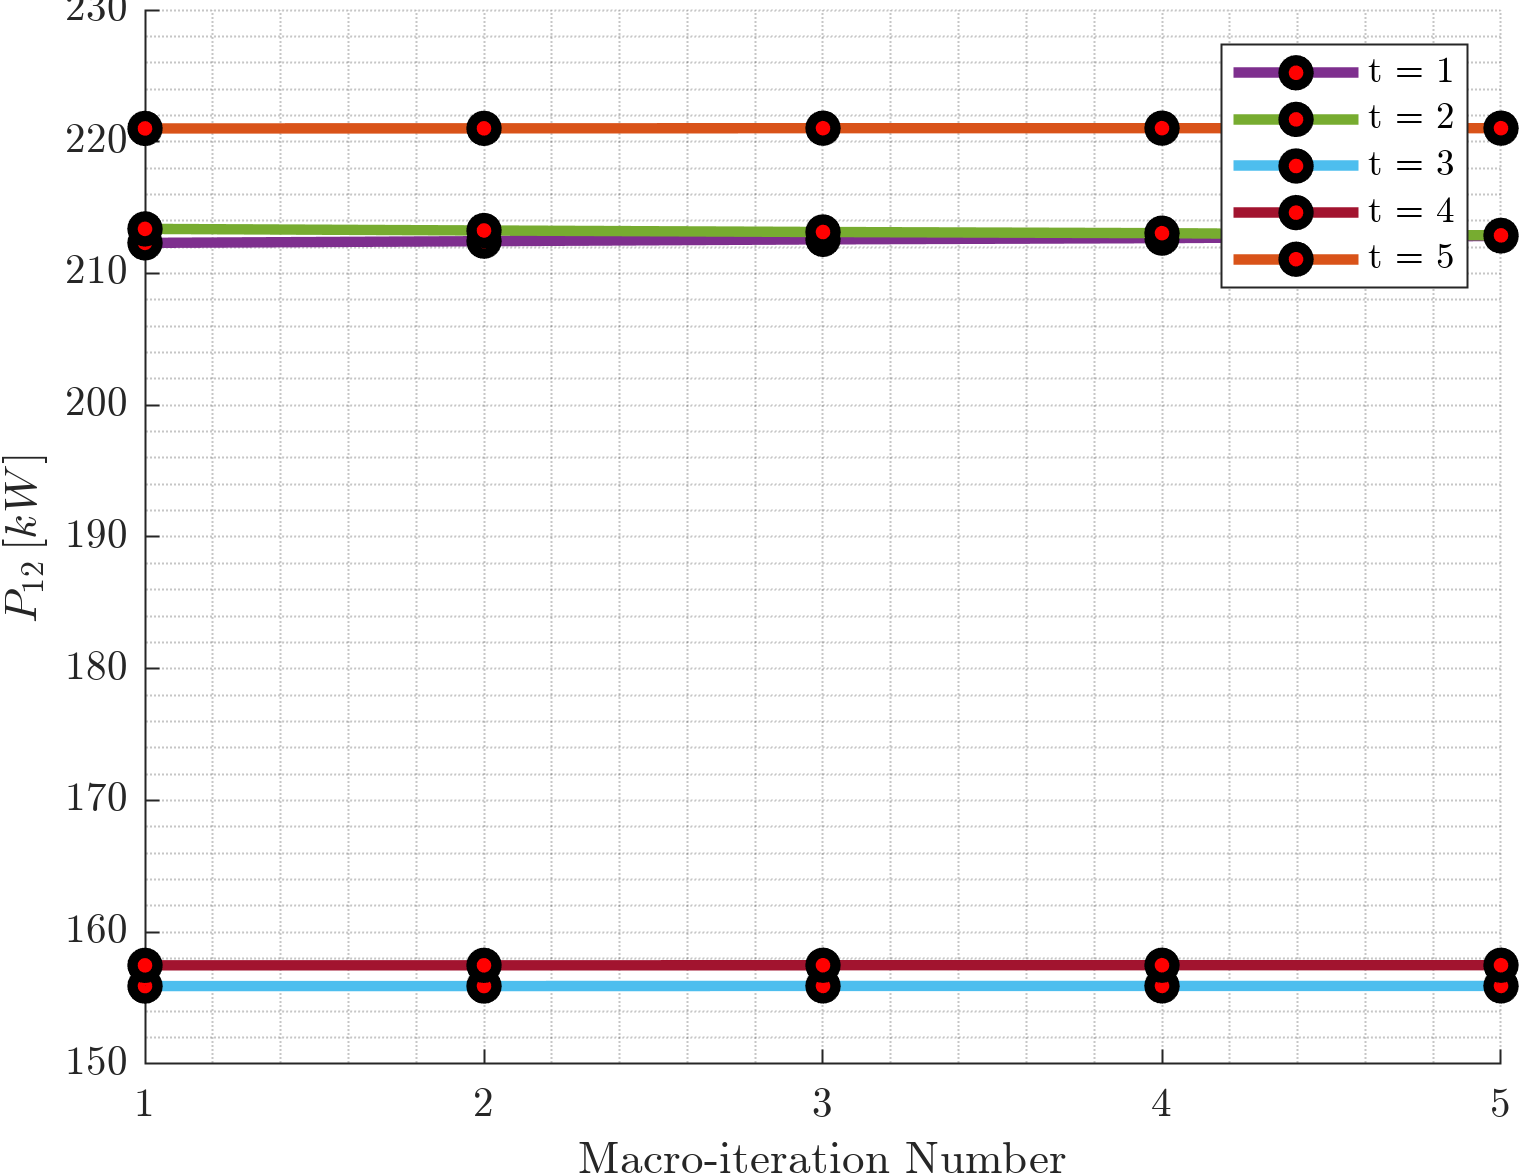
\includegraphics[width=\textwidth,height=0.6\textwidth]{../figures/T5-pv20-batt30-genCost/dopf/convergenceCurves/BoundaryRealPower_vs_t_vs_macroItr_T_5_Areas_1_3_genCost_pv_20_batt_30_crop.png}
%         \caption{\scriptsize Real Power flowing from Area $1$ into Area $3$}
%         \label{fig:real_power_1_3}
%     \end{subfigure}
%     \hfill
%     \begin{subfigure}[b]{0.3\textwidth}
%         \centering
%         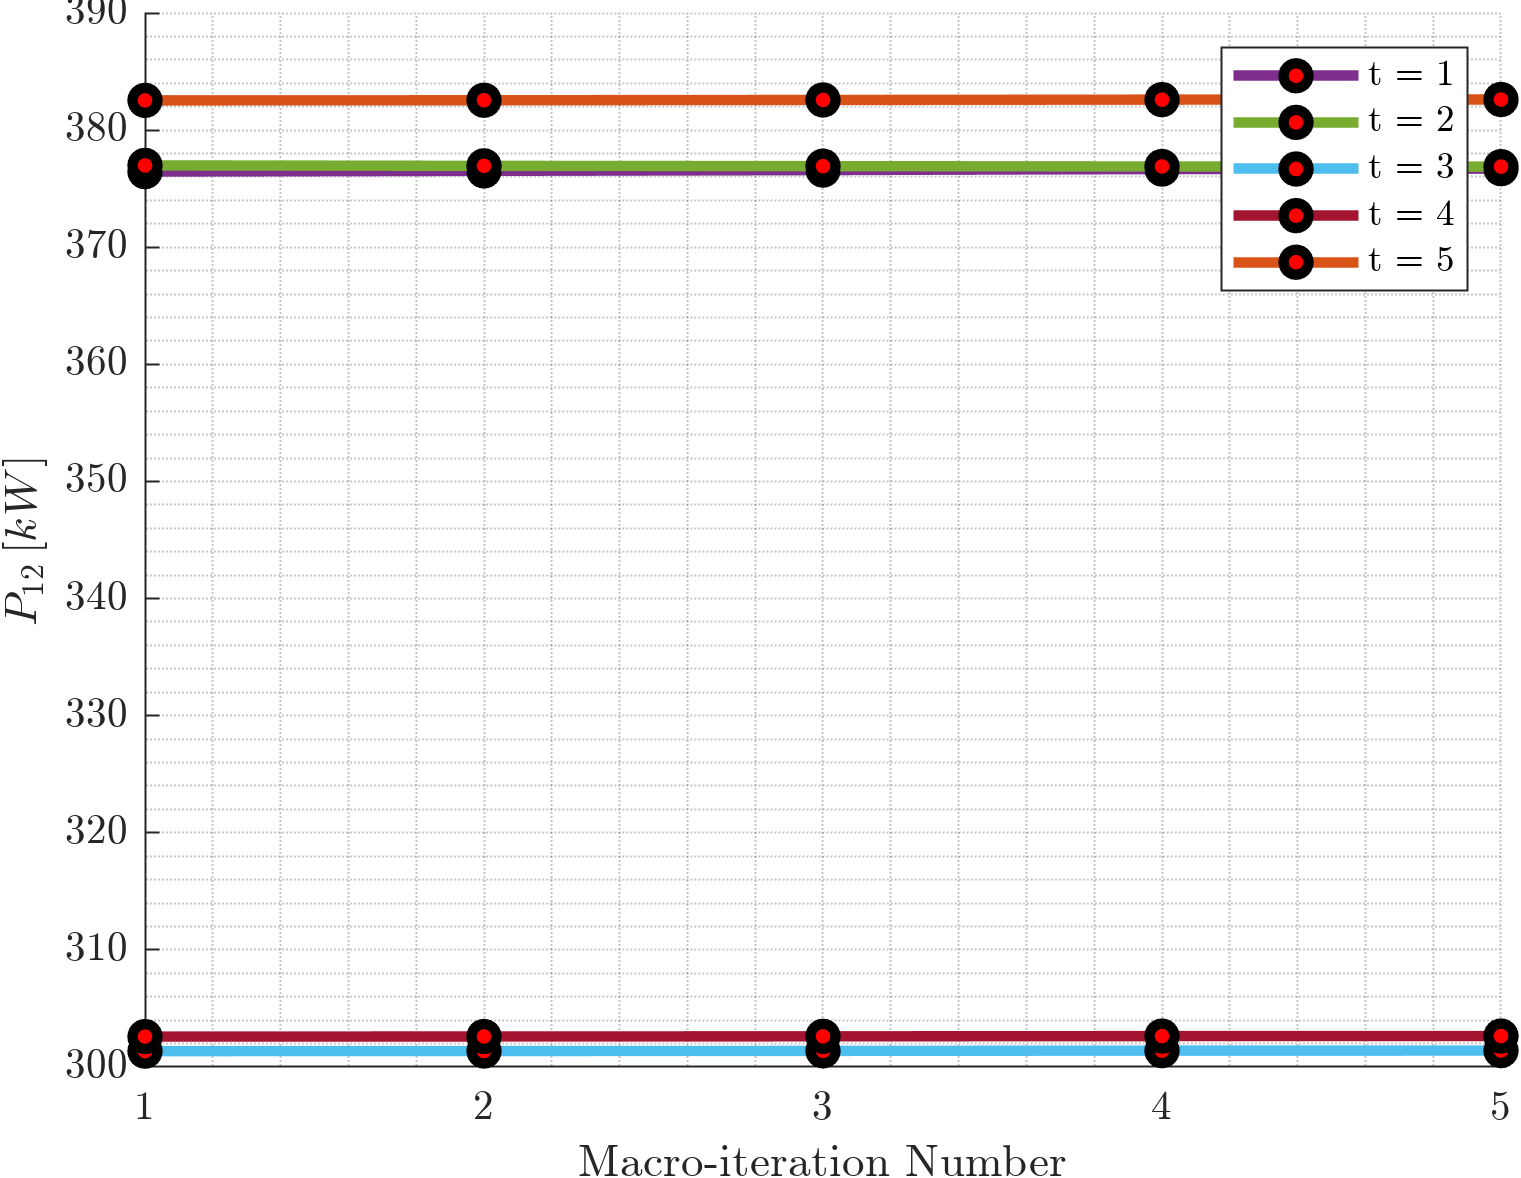
\includegraphics[width=\textwidth,height=0.6\textwidth]{../figures/T5-pv20-batt30-genCost/dopf/convergenceCurves/BoundaryRealPower_vs_t_vs_macroItr_T_5_Areas_2_4_genCost_pv_20_batt_30_crop.png}
%         \caption{\scriptsize Real Power flowing from Area $2$ into Area $4$}
%         \label{fig:real_power_2_4}
%     \end{subfigure}
    
%     % Row 2
%     \begin{subfigure}[b]{0.3\textwidth}
%         \centering
%         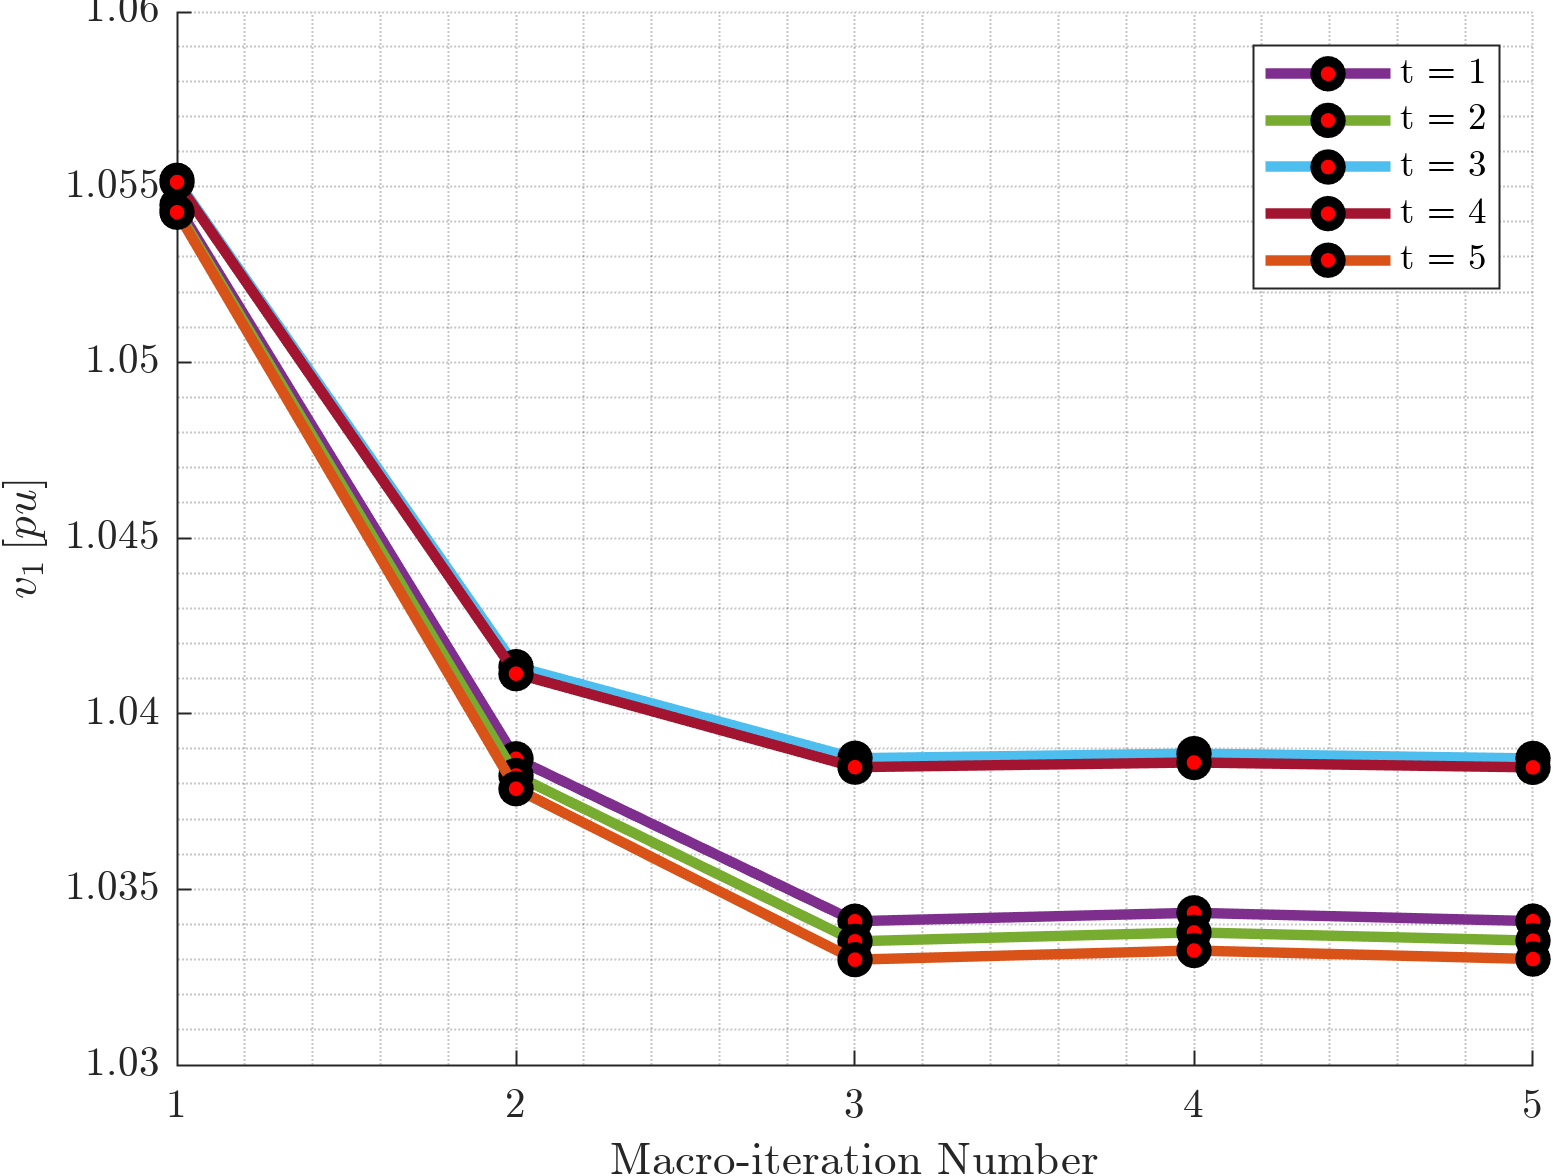
\includegraphics[width=\textwidth,height=0.6\textwidth]{../figures/T5-pv20-batt30-genCost/dopf/convergenceCurves/BoundaryVoltage_vs_t_vs_macroItr_T_5_Areas_1_2_genCost_pv_20_batt_30_crop.png}
%         \caption{\scriptsize Voltage at the PoI of Area $1$ and Area $2$}
%         \label{fig:voltage_1_2}
%     \end{subfigure}
%     \hfill
%     \begin{subfigure}[b]{0.3\textwidth}
%         \centering
%         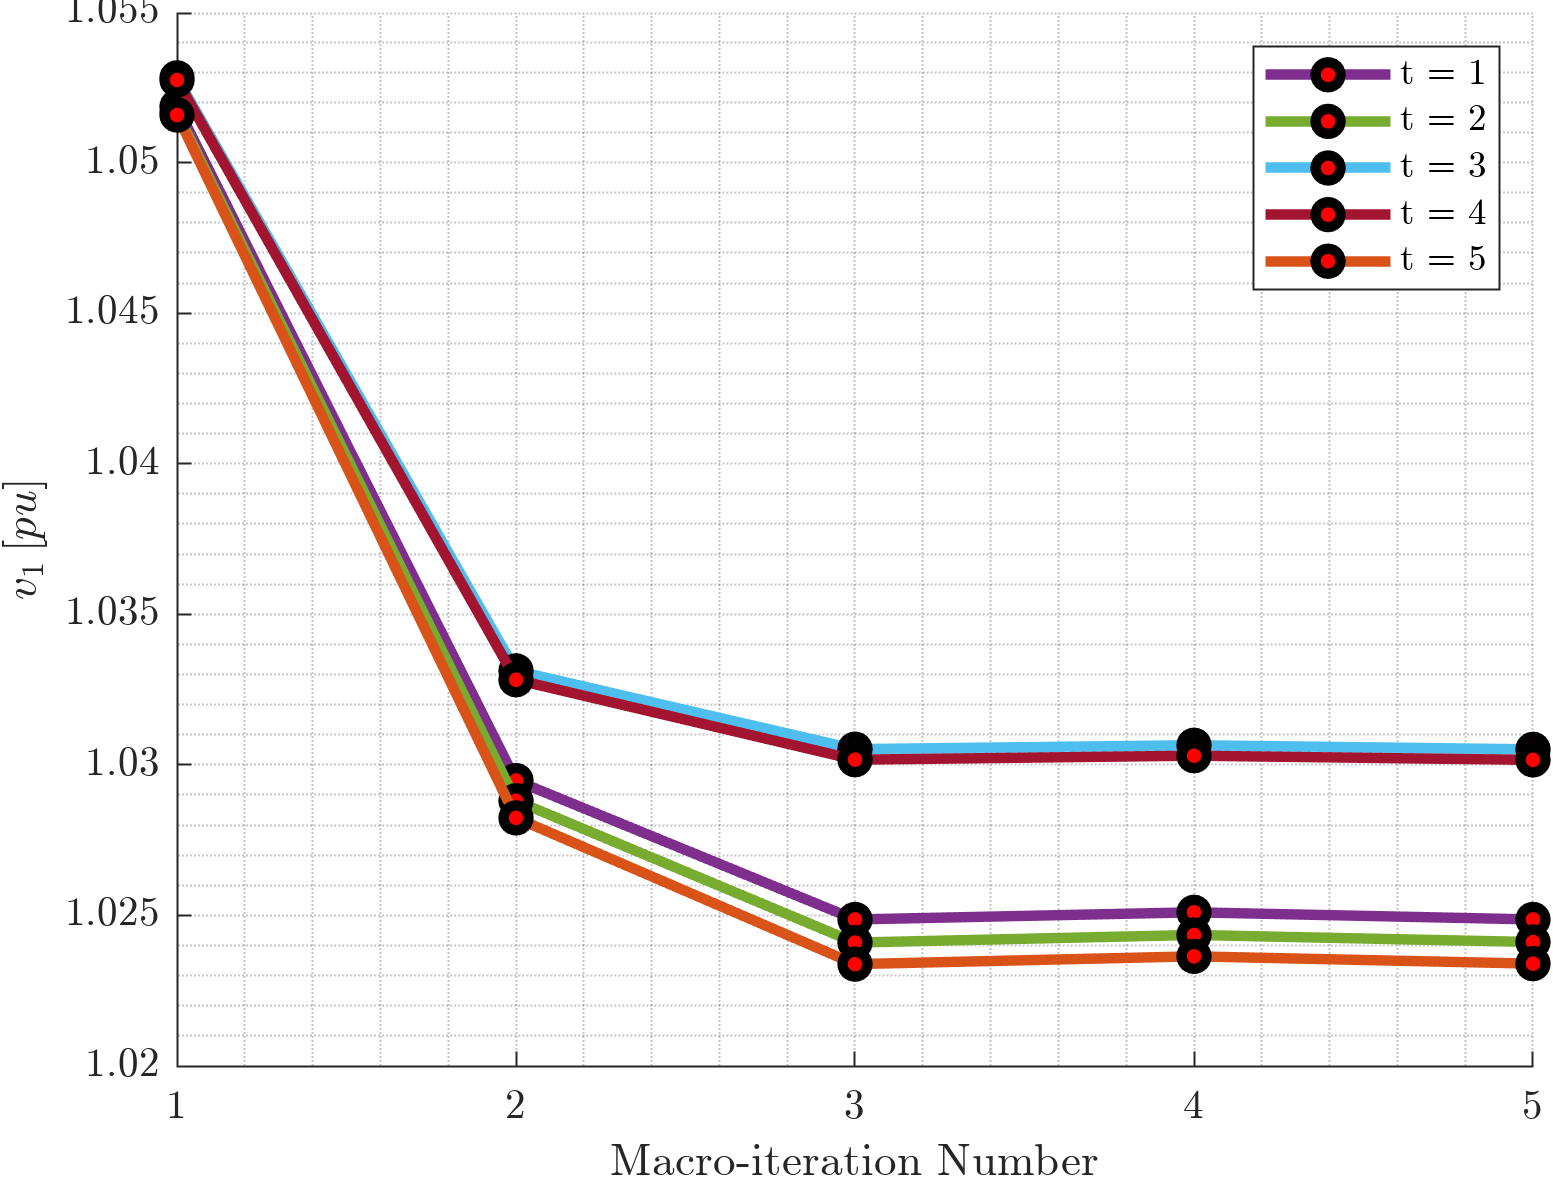
\includegraphics[width=\textwidth,height=0.6\textwidth]{../figures/T5-pv20-batt30-genCost/dopf/convergenceCurves/BoundaryVoltage_vs_t_vs_macroItr_T_5_Areas_1_3_genCost_pv_20_batt_30_crop.png}
%         \caption{\scriptsize Voltage at the PoI of Area $1$ and Area $3$}
%         \label{fig:voltage_1_3}
%     \end{subfigure}
%     \hfill
%     \begin{subfigure}[b]{0.3\textwidth}
%         \centering
%         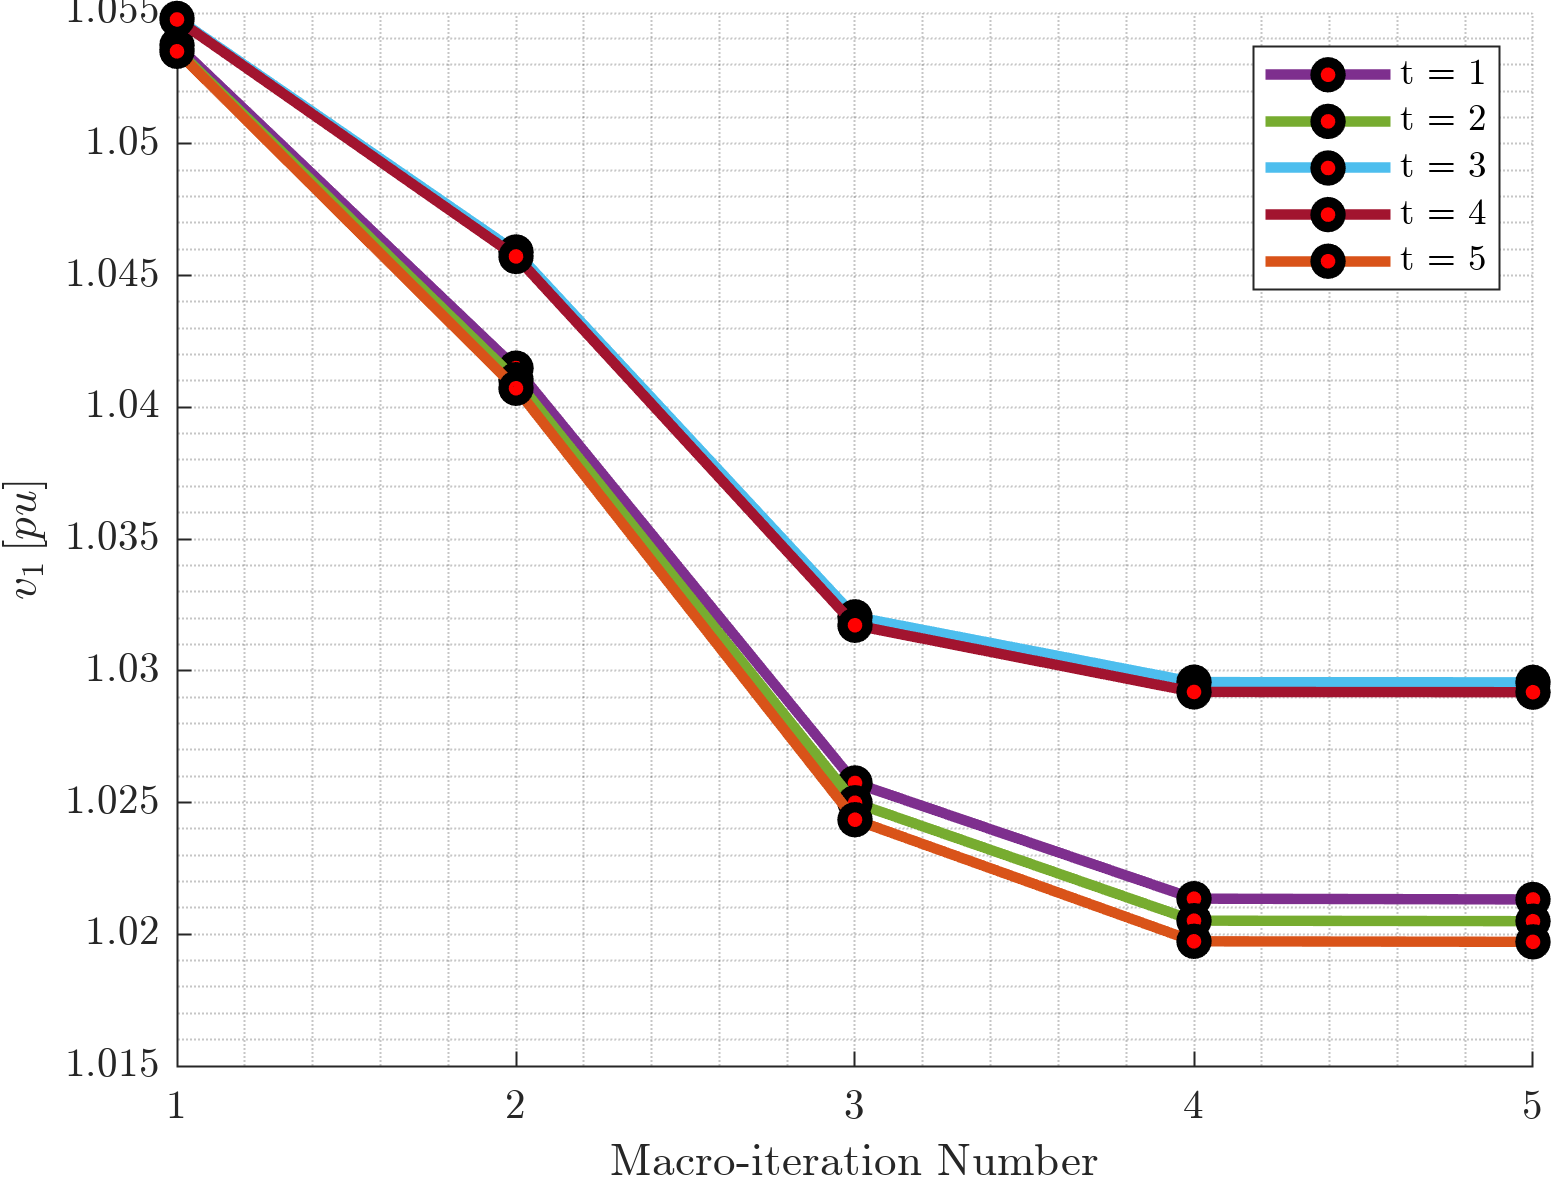
\includegraphics[width=\textwidth,height=0.6\textwidth]{../figures/T5-pv20-batt30-genCost/dopf/convergenceCurves/BoundaryVoltage_vs_t_vs_macroItr_T_5_Areas_2_4_genCost_pv_20_batt_30_crop.png}
%         \caption{\scriptsize Voltage at the PoI of Area $2$ and Area $4$}
%         \label{fig:voltage_2_4}
%     \end{subfigure}

%     \caption{Convergence of Boundary variables with every iteration. Each plot represents a particular variable exchanged between a pair of connected areas. Each line graph within a plot represents a particular time period.}
%     \label{fig:convergenceCurves-5-20-30}
% \end{figure}

% \begin{figure*}[h!] % convergence curves
%     \centering
%     % Row 1
%     \begin{subfigure}[t]{0.32\textwidth}
%         \centering
%         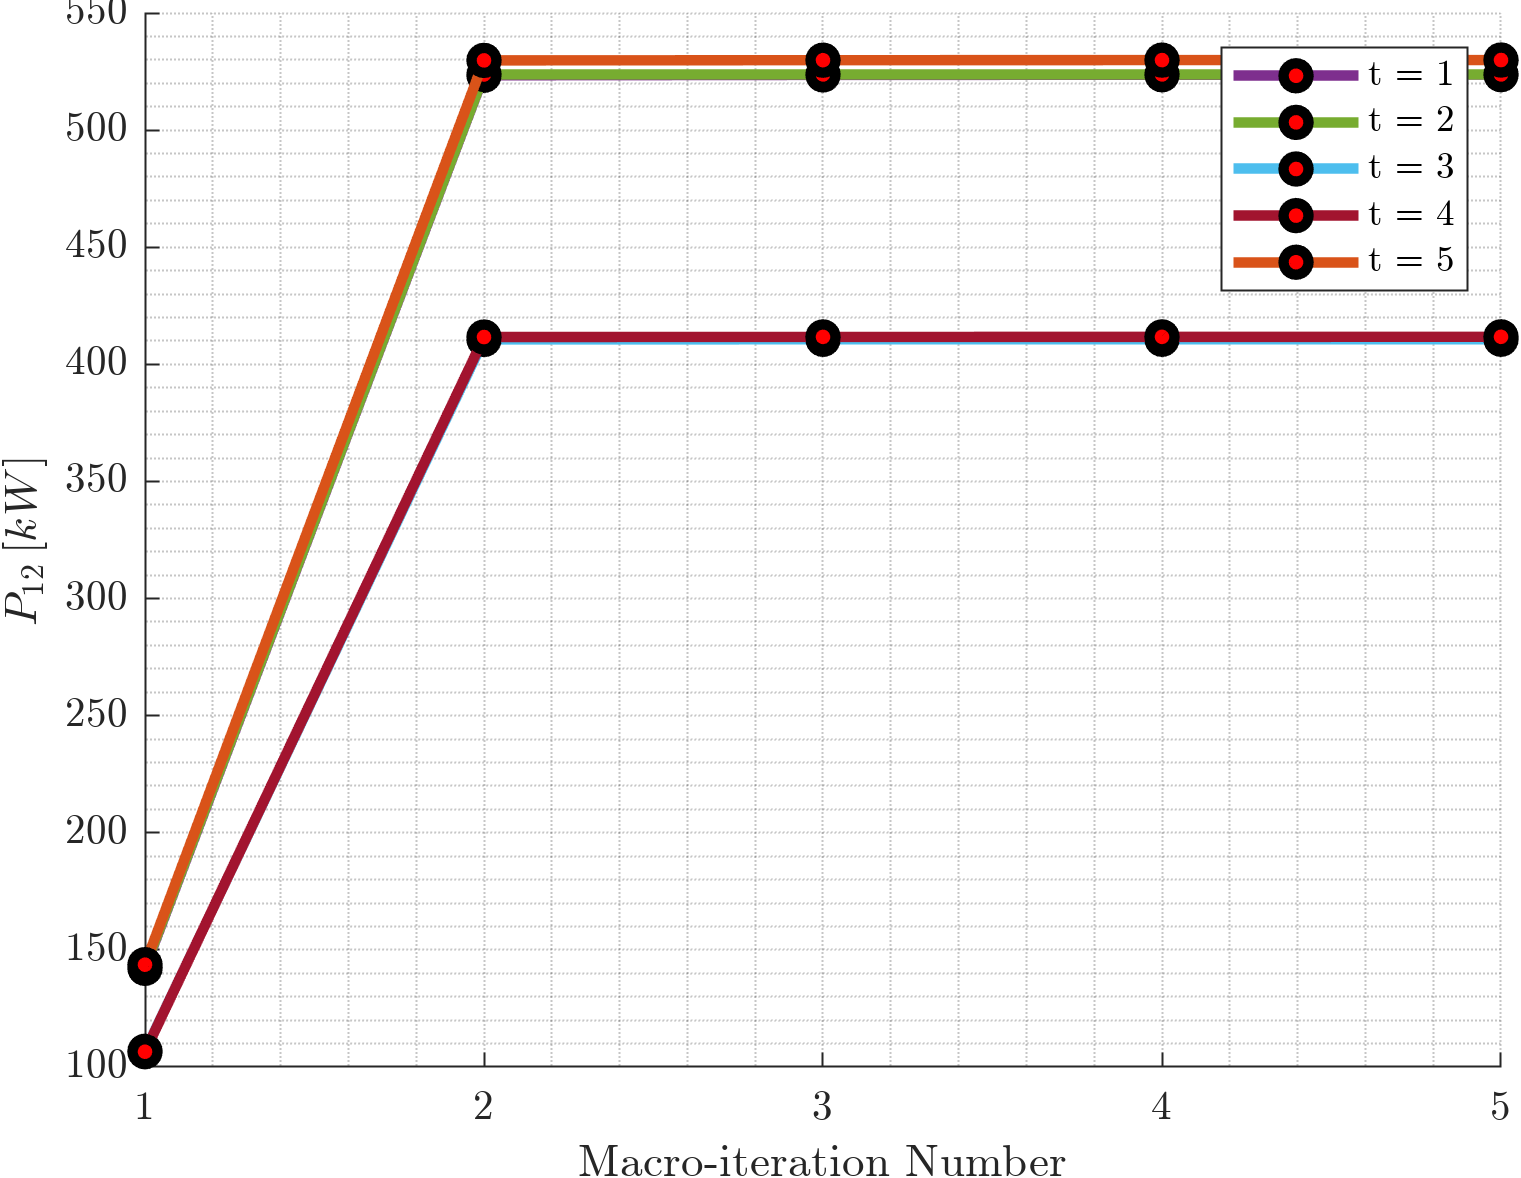
\includegraphics[width=\textwidth]{../figures/T5-pv20-batt30-genCost/dopf/convergenceCurves/BoundaryRealPower_vs_t_vs_macroItr_T_5_Areas_1_2_genCost_pv_20_batt_30_crop.png}
%         \caption{\scriptsize Real Power flowing from Area $1$ into Area $2$}
%         \label{fig:real_power_1_2}
%     \end{subfigure}
%     \hfill
%     \begin{subfigure}[t]{0.32\textwidth}
%         \centering
%         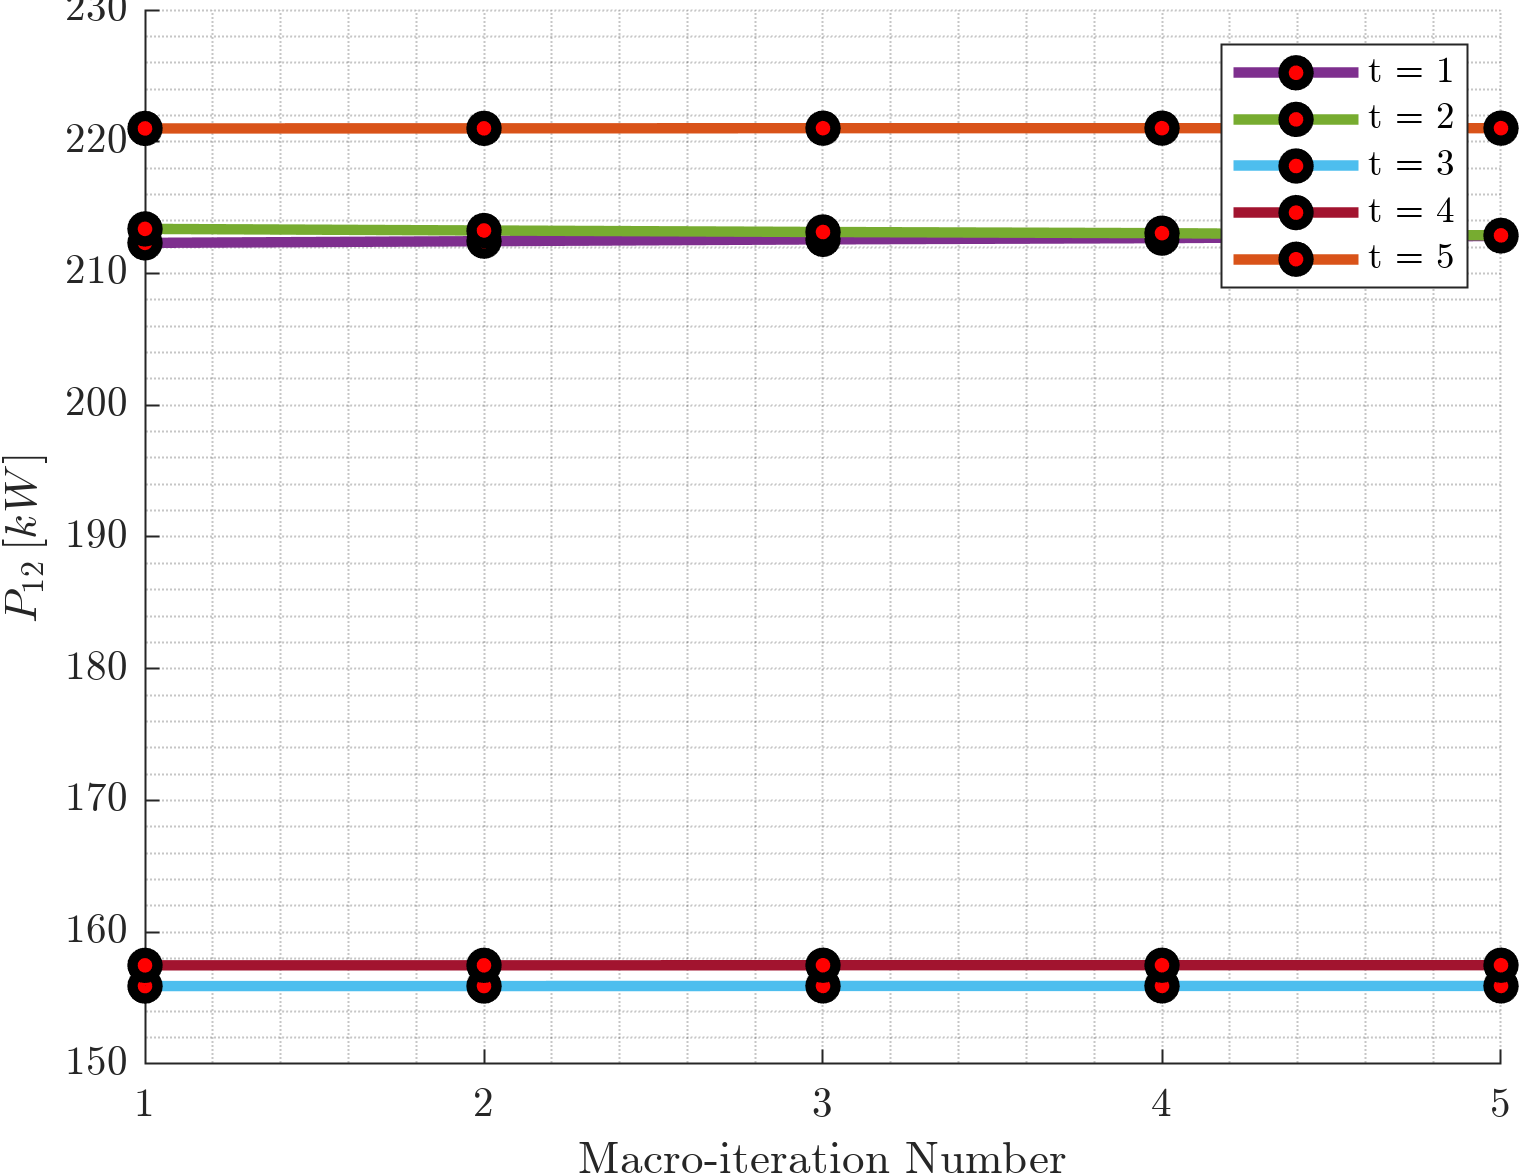
\includegraphics[width=\textwidth]{../figures/T5-pv20-batt30-genCost/dopf/convergenceCurves/BoundaryRealPower_vs_t_vs_macroItr_T_5_Areas_1_3_genCost_pv_20_batt_30_crop.png}
%         \caption{\scriptsize Real Power flowing from Area $1$ into Area $3$}
%         \label{fig:real_power_1_3}
%     \end{subfigure}
%     \hfill
%     \begin{subfigure}[t]{0.32\textwidth}
%         \centering
%         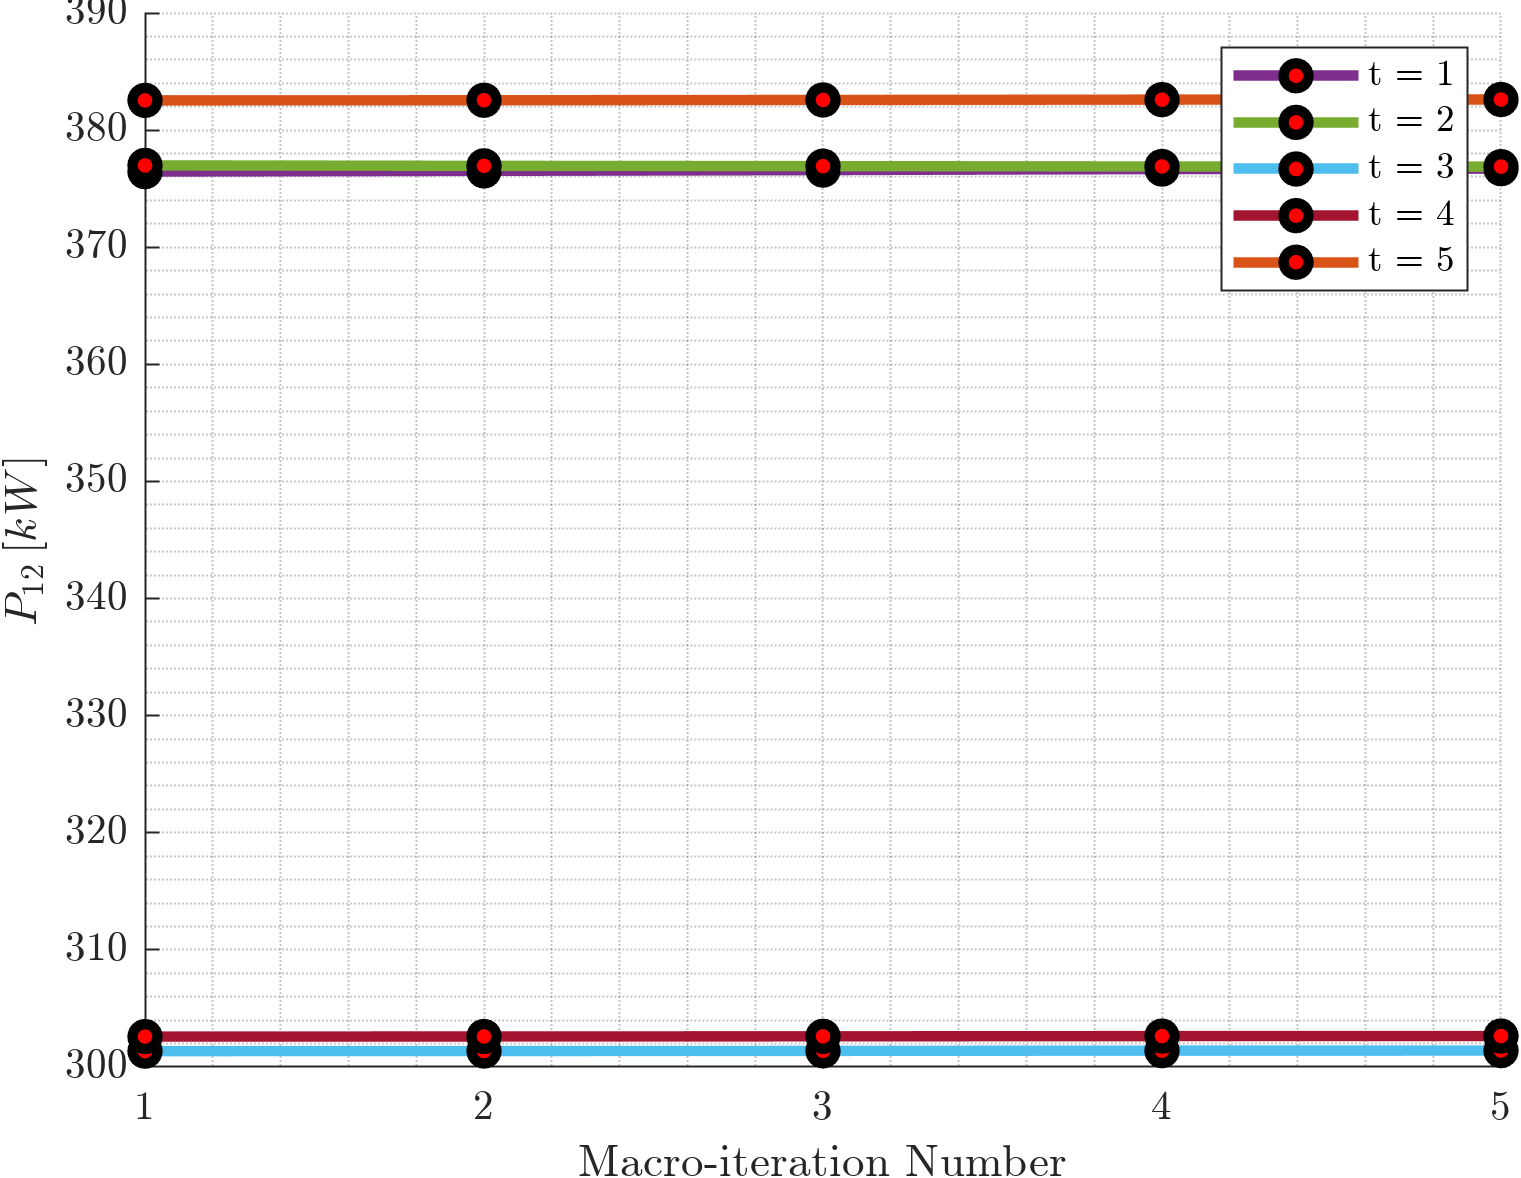
\includegraphics[width=\textwidth]{../figures/T5-pv20-batt30-genCost/dopf/convergenceCurves/BoundaryRealPower_vs_t_vs_macroItr_T_5_Areas_2_4_genCost_pv_20_batt_30_crop.png}
%         \caption{\scriptsize Real Power flowing from Area $2$ into Area $4$}
%         \label{fig:real_power_2_4}
%     \end{subfigure}
    
%     % Row 2
%     \begin{subfigure}[t]{0.32\textwidth}
%         \centering
%         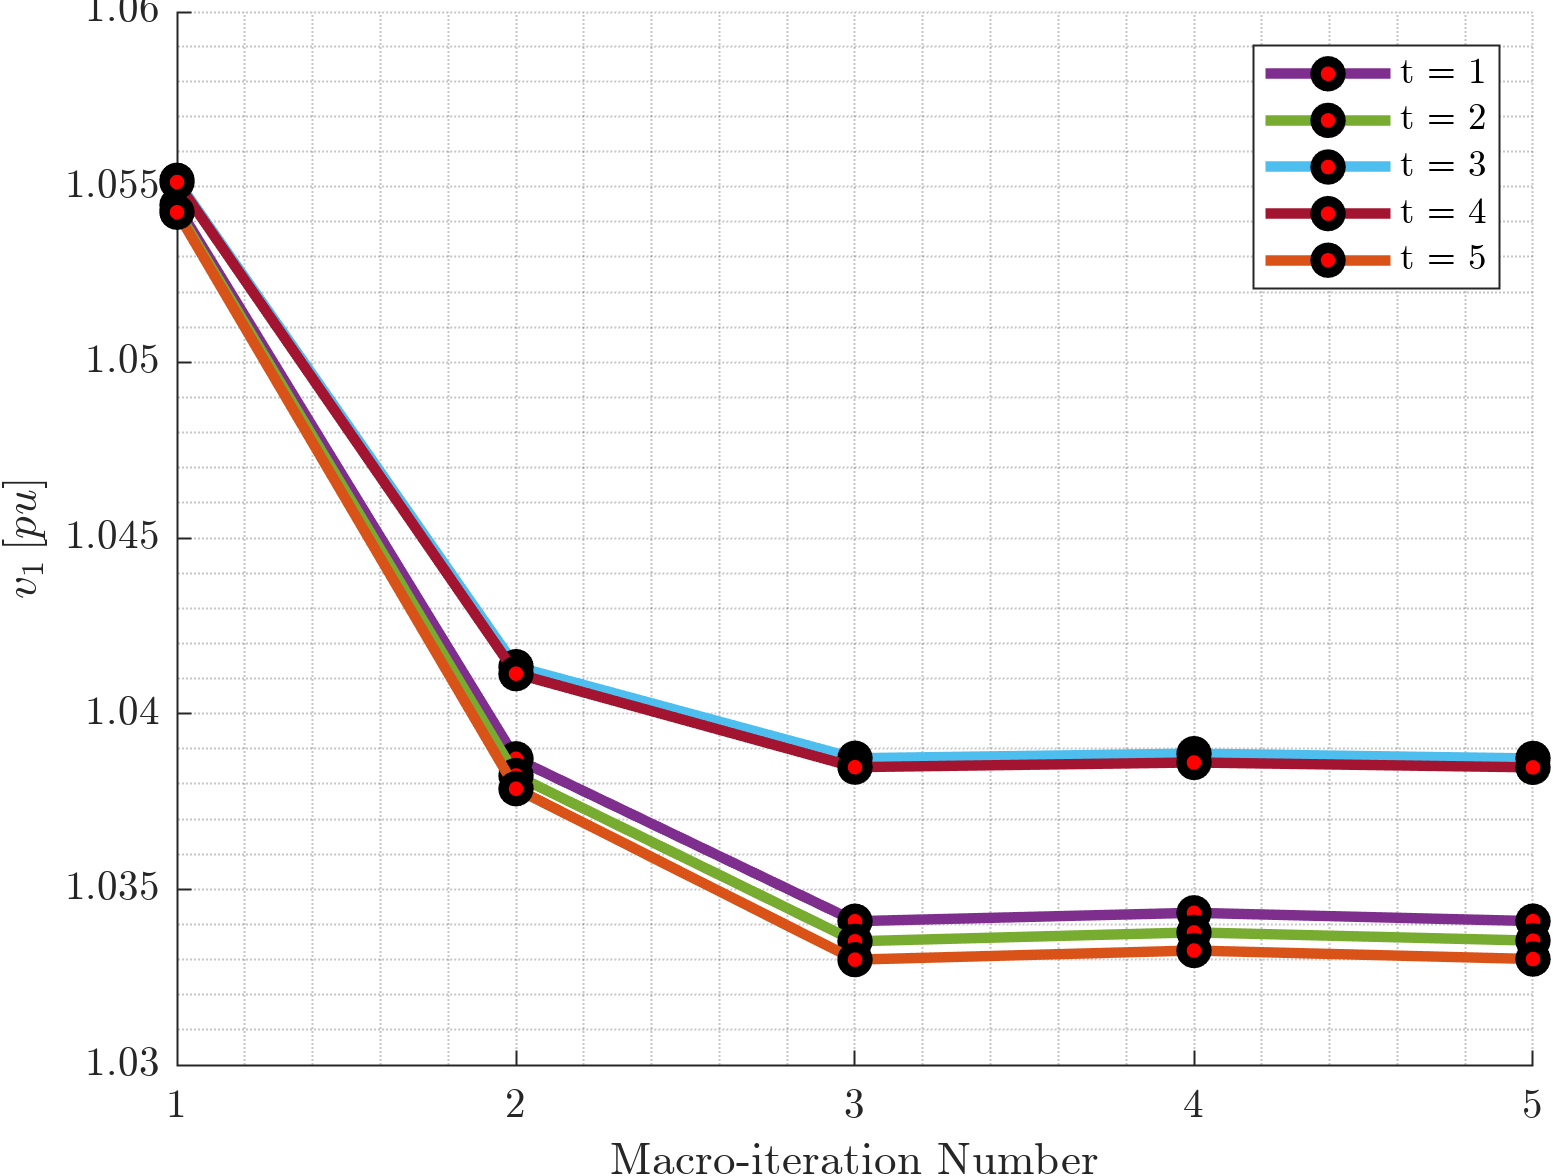
\includegraphics[width=\textwidth]{../figures/T5-pv20-batt30-genCost/dopf/convergenceCurves/BoundaryVoltage_vs_t_vs_macroItr_T_5_Areas_1_2_genCost_pv_20_batt_30_crop.png}
%         \caption{\scriptsize Voltage at the PoI of Area $1$ and Area $2$}
%         \label{fig:voltage_1_2}
%     \end{subfigure}
%     \hfill
%     \begin{subfigure}[t]{0.32\textwidth}
%         \centering
%         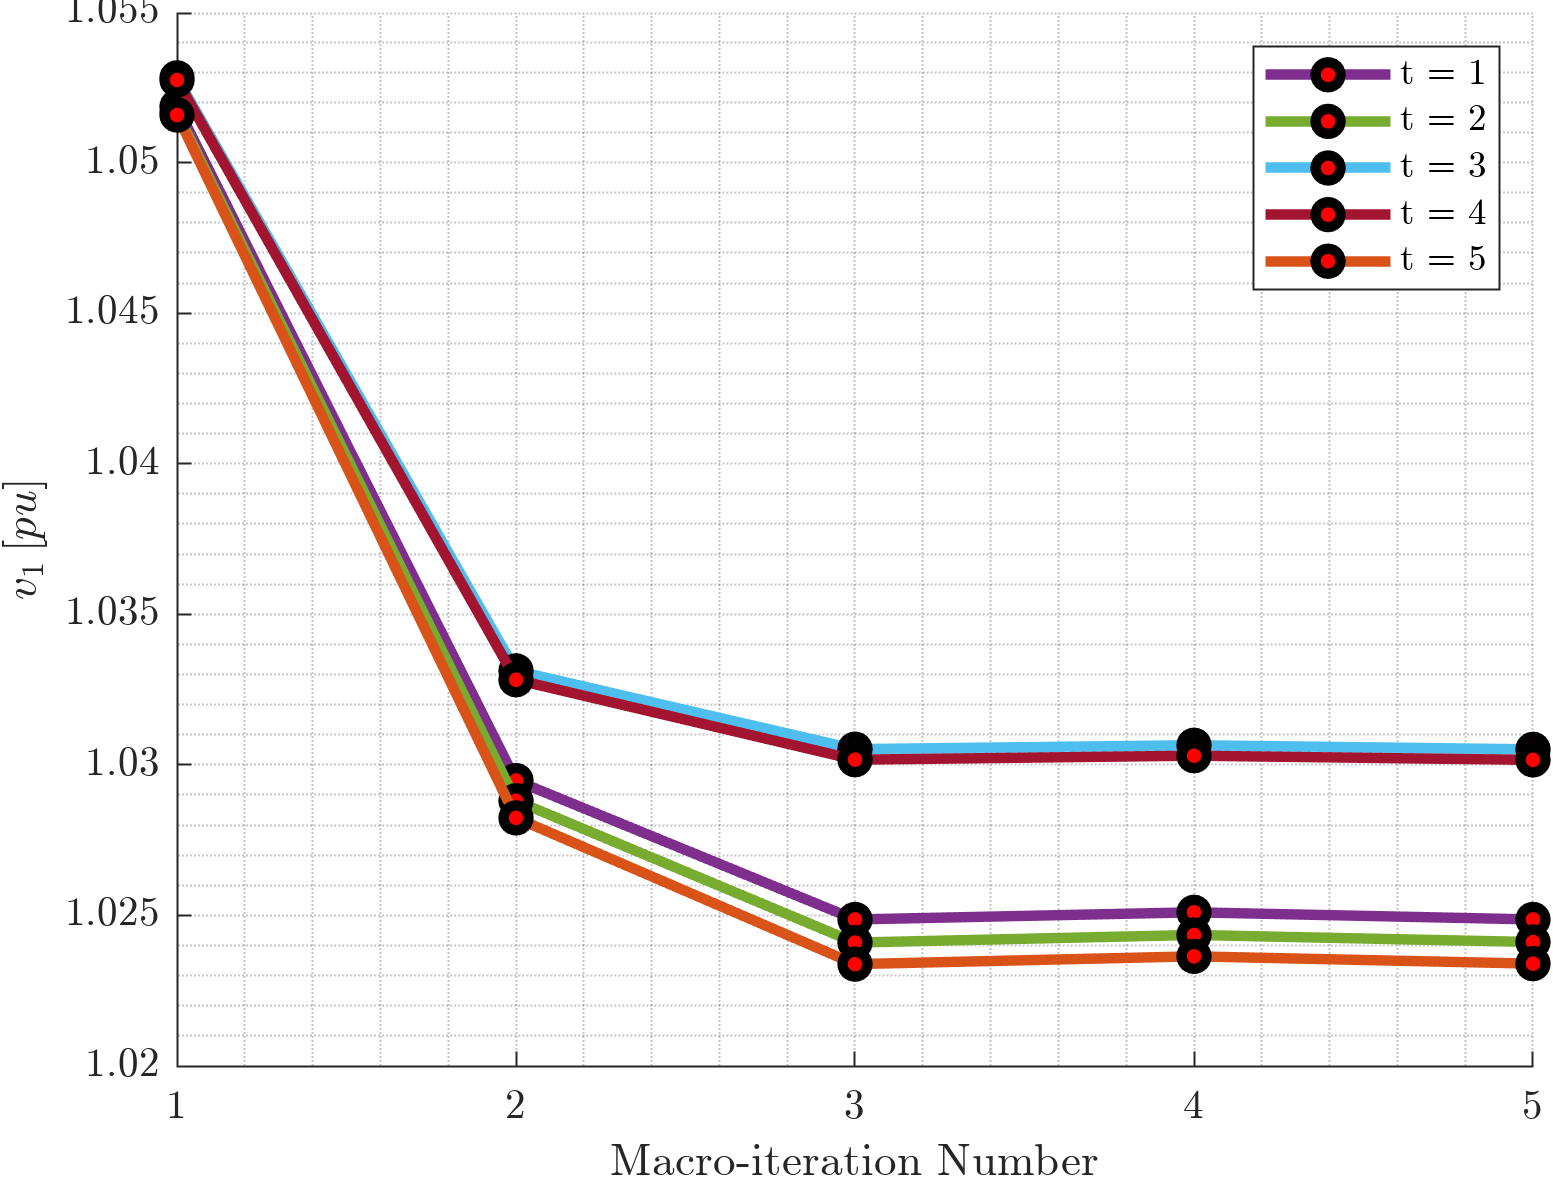
\includegraphics[width=\textwidth]{../figures/T5-pv20-batt30-genCost/dopf/convergenceCurves/BoundaryVoltage_vs_t_vs_macroItr_T_5_Areas_1_3_genCost_pv_20_batt_30_crop.png}
%         \caption{\scriptsize Voltage at the PoI of Area $1$ and Area $3$}
%         \label{fig:voltage_1_3}
%     \end{subfigure}
%     \hfill
%     \begin{subfigure}[t]{0.32\textwidth}
%         \centering
%         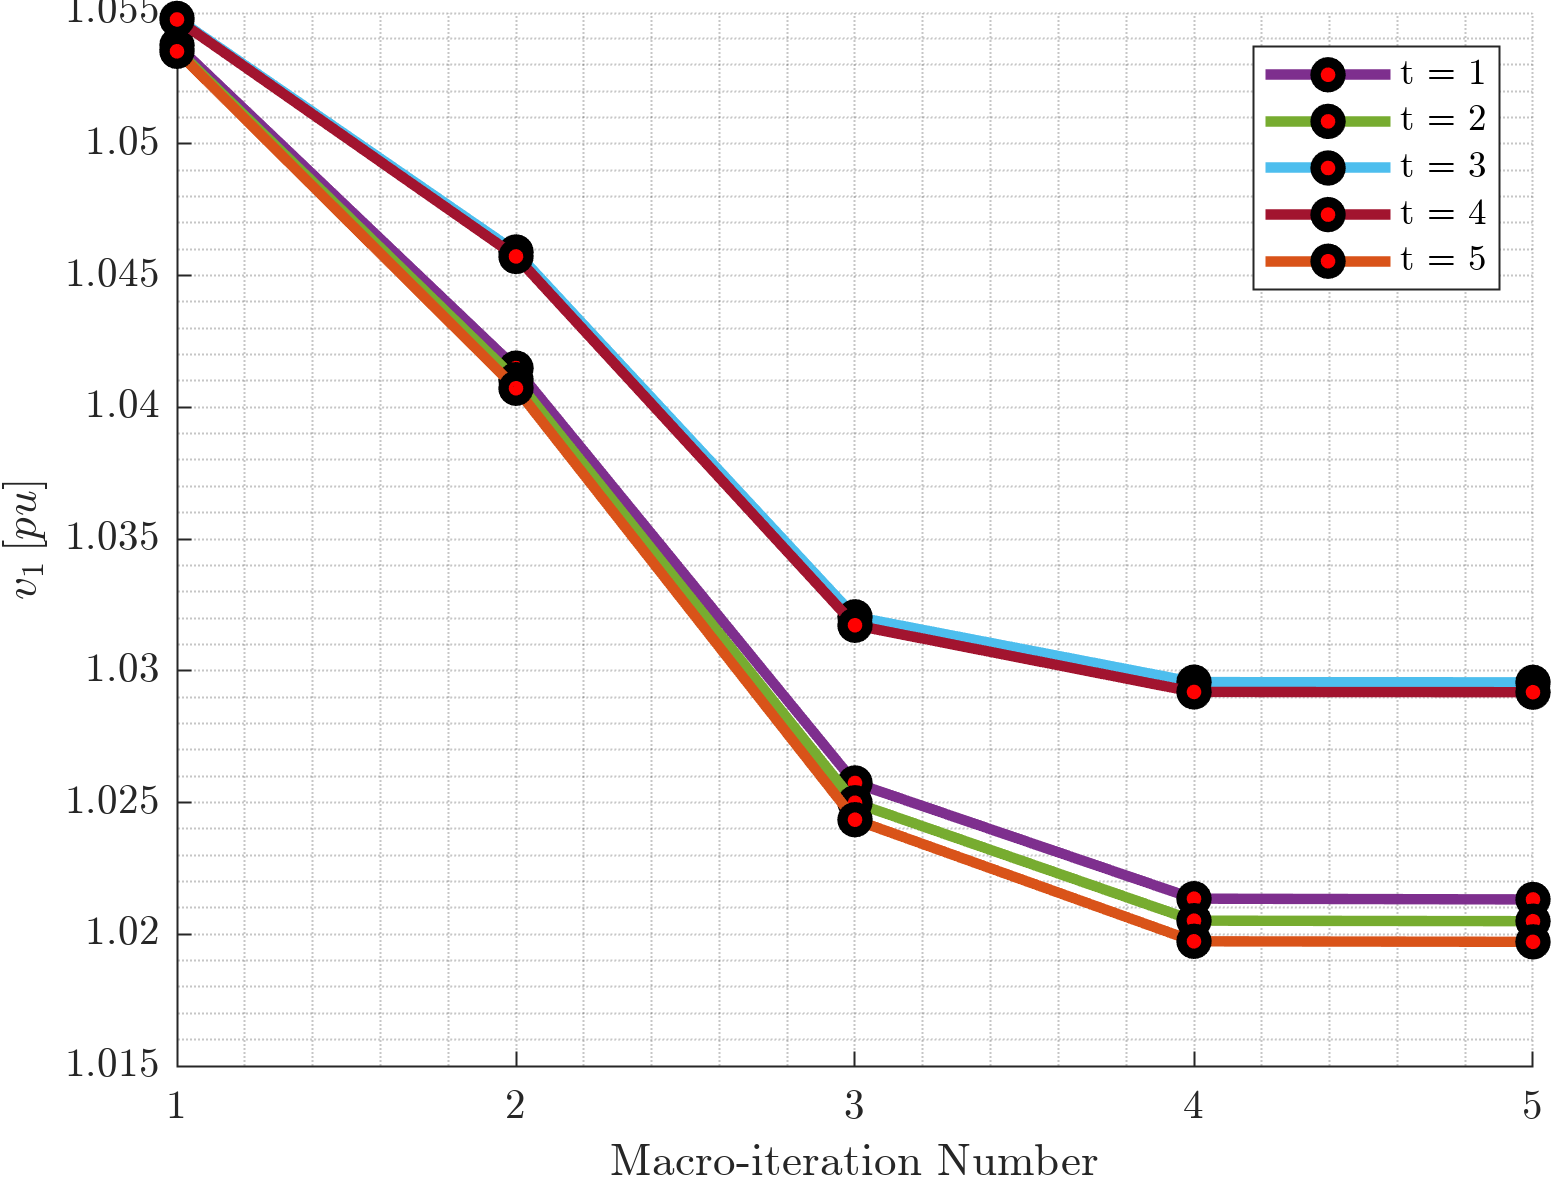
\includegraphics[width=\textwidth]{../figures/T5-pv20-batt30-genCost/dopf/convergenceCurves/BoundaryVoltage_vs_t_vs_macroItr_T_5_Areas_2_4_genCost_pv_20_batt_30_crop.png}
%         \caption{\scriptsize Voltage at the PoI of Area $2$ and Area $4$}
%         \label{fig:voltage_2_4}
%     \end{subfigure}

%     \caption{Convergence of Boundary variables with every iteration. Each plot represents a particular variable exchanged between a pair of connected areas. Each line graph within a plot represents a particular time period.}
%     \label{fig:convergenceCurves-5-20-30}
% \end{figure*}

\begin{figure}[h!]
    \centering
    % First plot: Voltage at the PoI of Area 1 and Area 2
    \begin{subfigure}[b]{\columnwidth}
        \centering
        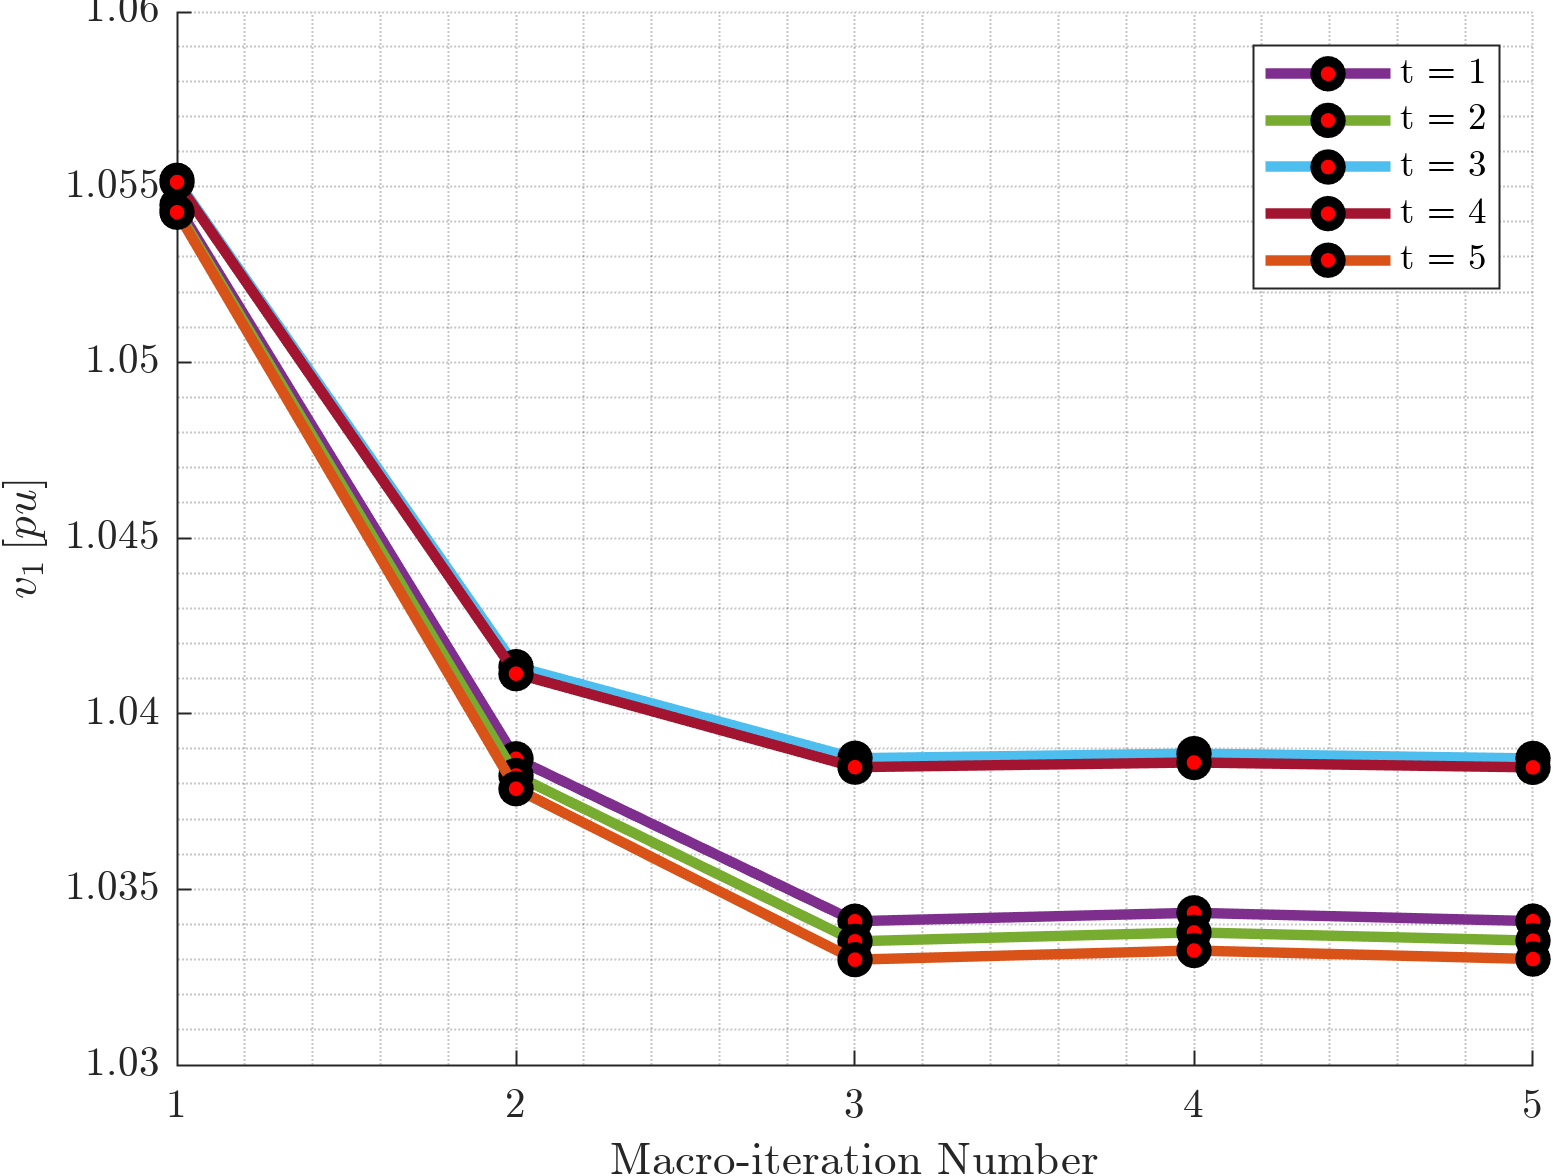
\includegraphics[width=0.8\columnwidth]{../figures/T5-pv20-batt30-genCost/dopf/convergenceCurves/BoundaryVoltage_vs_t_vs_macroItr_T_5_Areas_1_2_genCost_pv_20_batt_30_crop.png}
        \caption{\scriptsize Voltage at the Point of Interconnection of Area $1$ and Area $2$}
        \label{fig:voltage_1_2}
    \end{subfigure}
    \vfill
    % Second plot: Real Power flowing from Area 2 into Area 4
    \begin{subfigure}[b]{\columnwidth}
        \centering
        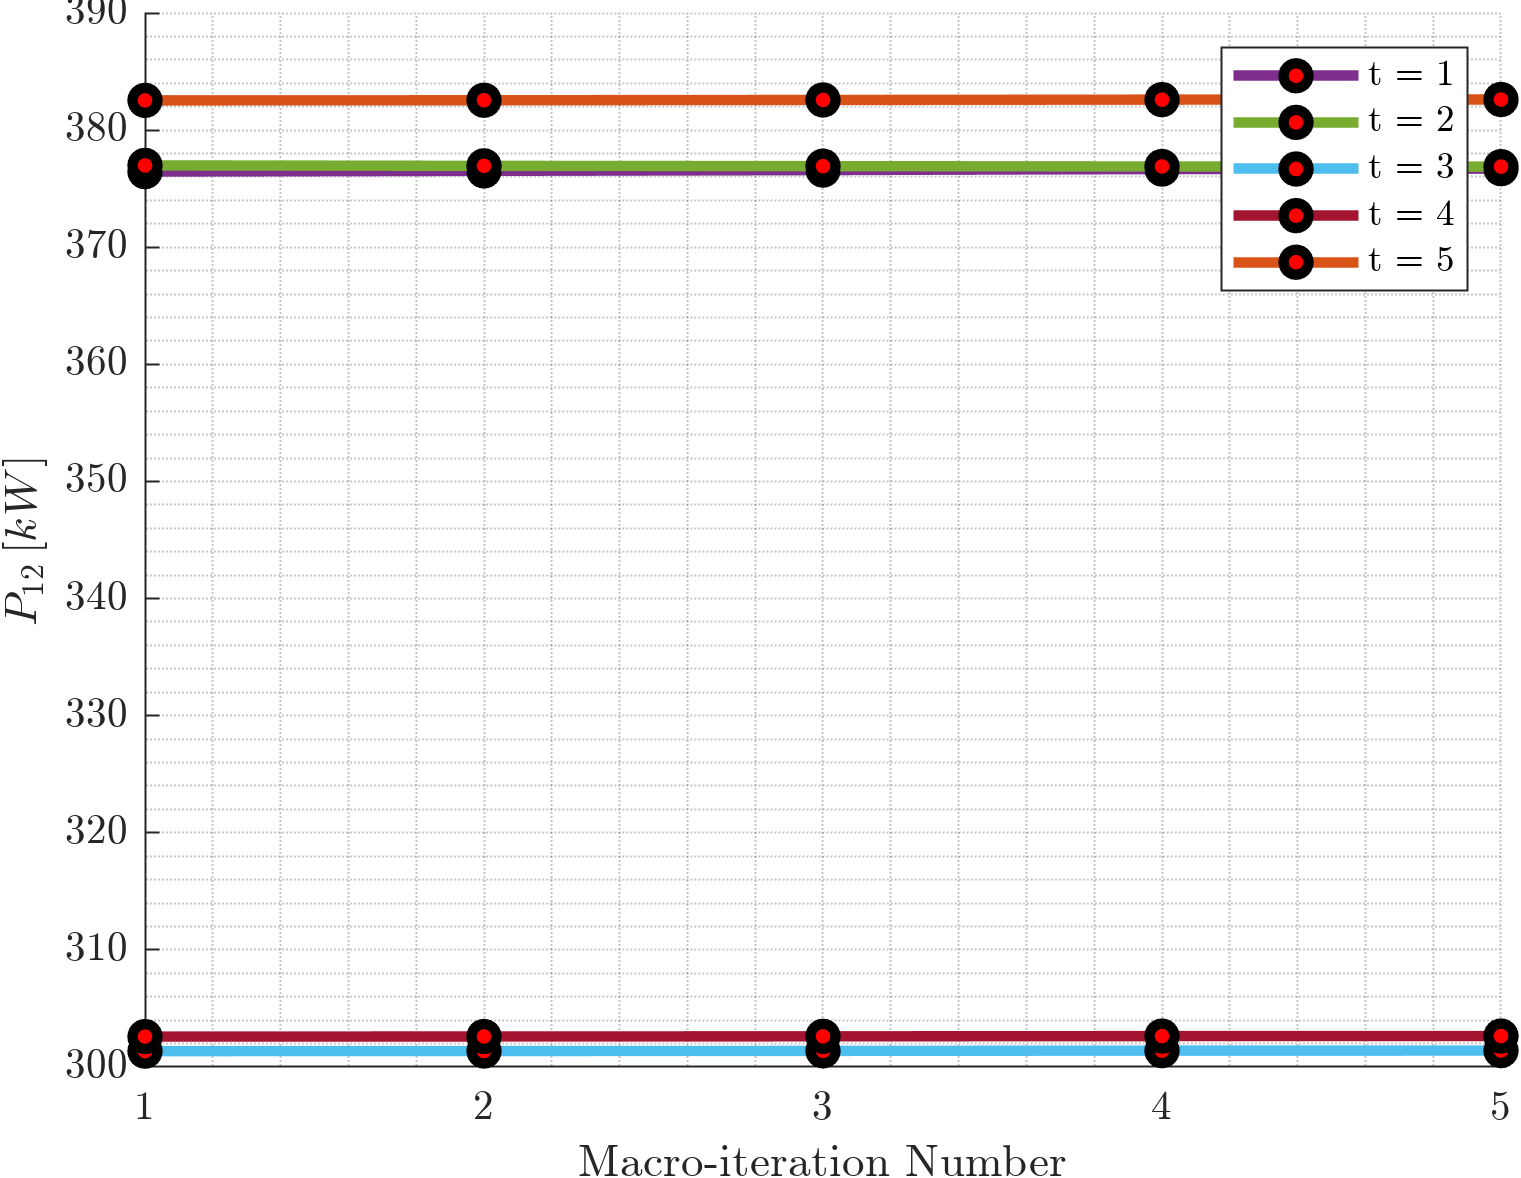
\includegraphics[width=0.8\columnwidth]{../figures/T5-pv20-batt30-genCost/dopf/convergenceCurves/BoundaryRealPower_vs_t_vs_macroItr_T_5_Areas_2_4_genCost_pv_20_batt_30_crop.png}
        \caption{\scriptsize Real Power flowing from Area $2$ into Area $4$}
        \label{fig:real_power_2_4}
    \end{subfigure}
    
    \caption{Convergence of Boundary variables with every iteration. Each plot represents a particular variable exchanged between a pair of connected areas. Each line graph within a plot represents a particular time period.}
    \label{fig:convergenceCurves-5-20-30}
\end{figure}


Similarly, the convergence of the objective function to its optimal value with every iteration is shown by \Cref{fig:outputConvergence-5-pv20-batt30-genCost}.

\begin{figure}[h!] % output variable convergence curve
    \centering
    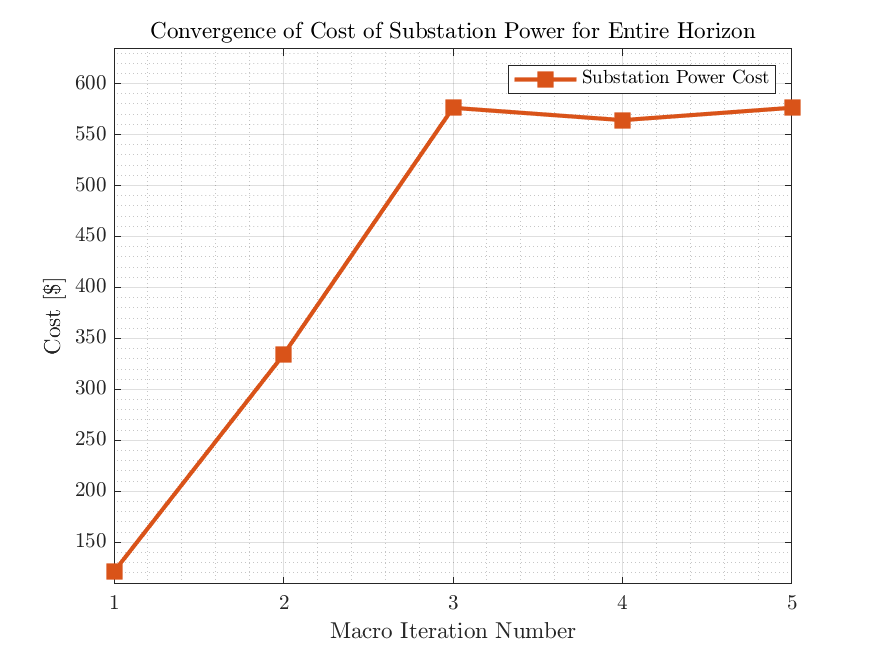
\includegraphics[height=0.25\textheight]{../figures/T5-pv20-batt30-genCost/dopf/outputCurves/ObjectiveConvergenceCurves_Horizon_5.png}
    \caption{Convergence of Objective Function Value with each MPDOPF iteration}
    \label{fig:outputConvergence-5-pv20-batt30-genCost}
\end{figure}

\subsection{Scalability Analysis} \label{subsec:scalabilityAnalysis}

To demonstrate the effectiveness of the proposed algorithm over a bigger horizon to demonstrate scalability, simulations were run for a $10$ time-period horizon. \Cref{fig:inputCurve-10} shows the forecasted profiles for load, solar irradiance and cost of substation power over the horizon. 

\begin{figure}[h!]
    \centering
    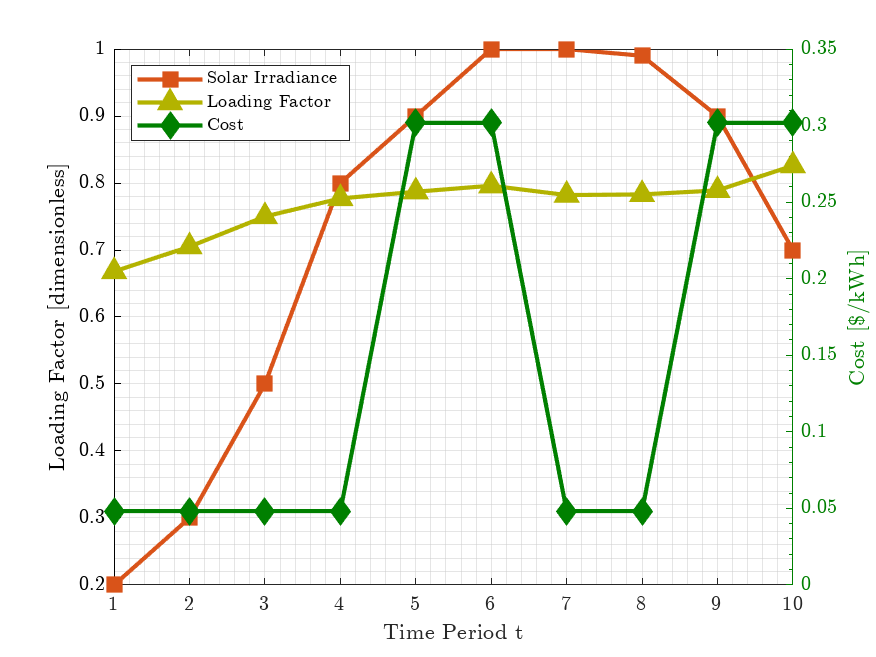
\includegraphics[height=0.25\textheight]{../figures/T10-inputCurves/InputCurves_Horizon_10.png}
    \caption{Forecasts for Demand Power, Irradiance and Cost of Substation Power over a 10 Hour Horizon}
    \label{fig:inputCurve-10}
\end{figure}

From the comparison against MPCOPF in \Cref{table:opt-10-20-30}, it can again be seen that MPDOPF is able to converge to the same optimal solution as MPCOPF. The computational speed up is even more pronounced than for the $5$ time-period simulation.

\begin{table}[H]
    \centering
    \caption{Comparative analyses between MPCOPF and MPDOPF - $10$ time-period horizon}
    \begin{tabular}{|l|c|c|}
    \hline
    \textbf{Metric} & \textbf{MPCOPF} & \textbf{MPDOPF} \\ \hline
    Biggest subproblem & \multicolumn{2}{c|}{} \\ \hline
    \quad Decision variables & {6300} & {2640} \\ \hline
    \quad Linear constraints & {11636} & {4891} \\ \hline
    \quad Nonlinear constraints & {1270} & {530} \\ \hline
    Simulation results  & \multicolumn{2}{c|}{} \\ \hline
    \quad Substation power cost (\$) & 1197.87 & 1197.87 \\ \hline
    \quad Substation real power (kW) & 8544.28 & 8544.04 \\ \hline
    \quad Line loss (kW) & 148.67 & 148.94 \\ \hline
    \quad Substation reactive power (kVAR) & 1092.39 & 1252.03 \\ \hline
    \quad PV reactive power (kVAR) & 222.59 & 139.81 \\ \hline
    \quad Battery reactive power (kVAR) & 388.52 & 310.94 \\ \hline
    Computation  & \multicolumn{2}{c|}{} \\ \hline
    \quad Number of Iterations & - & 5 \\ \hline
    \quad Total Simulation Time (s) & 4620.73 & 358.69 \\ \hline
    \end{tabular}
    \label{table:opt-10-20-30}
\end{table}


Again, comparison against OpenDSS has yielded small discrepancies, attesting to the feasiblity of the solution. 

\begin{table}[H]
    \centering
    \caption{ACOPF feasibility analyses - $10$ time-period horizon}
    \begin{tabular}{|l|c|c|}
    \hline
    \textbf{Metric} & \textbf{MPDOPF} & \textbf{OpenDSS} \\ \hline
    Full horizon  & \multicolumn{2}{c|}{} \\ \hline
    \quad Substation real power (kW) & 8544.04 & 8544.40 \\ \hline
    \quad Line loss (kW) & 148.94 & 148.87 \\ \hline
    \quad Substation reactive power (kVAR) & 1252.03 & 1243.36 \\ \hline
    Max. all-time discrepancy & \multicolumn{2}{c|}{} \\ \hline
    \quad Voltage (pu) & \multicolumn{2}{c|}{0.0002} \\ \hline
    \quad Line loss (kW) & \multicolumn{2}{c|}{0.0132} \\ \hline
    \quad Substation power (kW) & \multicolumn{2}{c|}{0.4002} \\ \hline
    \end{tabular}
    \label{table:feas-copf-10-20-30}
\end{table}

% \begin{figure}[h!]
%     \centering
%     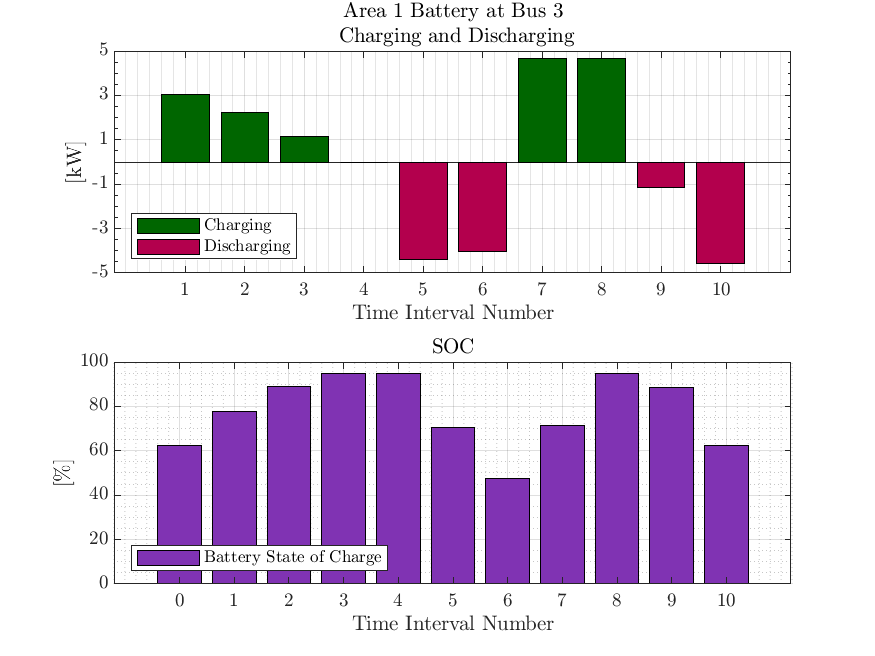
\includegraphics[width=\linewidth]{../figures/T10-pv20-batt30-genCost/dopf/BatteryPlots/macroItr_5_genCost_Battery_1_alpha_0.001.png}
%     \caption{Charging-Discharging and SOC graphs for Battery at Bus 3 located in Area 1 obtained via MPDOPF}
%     \label{fig:batt-plot-dopf-10-20-30-genCost}
% \end{figure}


\end{document}
